\documentclass[twoside]{book}

% Packages required by doxygen
\usepackage{fixltx2e}
\usepackage{calc}
\usepackage{doxygen}
\usepackage{graphicx}
\usepackage[utf8]{inputenc}
\usepackage{makeidx}
\usepackage{multicol}
\usepackage{multirow}
\PassOptionsToPackage{warn}{textcomp}
\usepackage{textcomp}
\usepackage[nointegrals]{wasysym}
\usepackage[table]{xcolor}

% NLS support packages
\usepackage{hfont}

% Font selection
\usepackage[T1]{fontenc}
\usepackage{mathptmx}
\usepackage[scaled=.90]{helvet}
\usepackage{courier}
\usepackage{amssymb}
\usepackage{sectsty}
\renewcommand{\familydefault}{\sfdefault}
\allsectionsfont{%
  \fontseries{bc}\selectfont%
  \color{darkgray}%
}
\renewcommand{\DoxyLabelFont}{%
  \fontseries{bc}\selectfont%
  \color{darkgray}%
}
\newcommand{\+}{\discretionary{\mbox{\scriptsize$\hookleftarrow$}}{}{}}

% Page & text layout
\usepackage{geometry}
\geometry{%
  a4paper,%
  top=2.5cm,%
  bottom=2.5cm,%
  left=2.5cm,%
  right=2.5cm%
}
\tolerance=750
\hfuzz=15pt
\hbadness=750
\setlength{\emergencystretch}{15pt}
\setlength{\parindent}{0cm}
\setlength{\parskip}{0.2cm}
\makeatletter
\renewcommand{\paragraph}{%
  \@startsection{paragraph}{4}{0ex}{-1.0ex}{1.0ex}{%
    \normalfont\normalsize\bfseries\SS@parafont%
  }%
}
\renewcommand{\subparagraph}{%
  \@startsection{subparagraph}{5}{0ex}{-1.0ex}{1.0ex}{%
    \normalfont\normalsize\bfseries\SS@subparafont%
  }%
}
\makeatother

% Headers & footers
\usepackage{fancyhdr}
\pagestyle{fancyplain}
\fancyhead[LE]{\fancyplain{}{\bfseries\thepage}}
\fancyhead[CE]{\fancyplain{}{}}
\fancyhead[RE]{\fancyplain{}{\bfseries\leftmark}}
\fancyhead[LO]{\fancyplain{}{\bfseries\rightmark}}
\fancyhead[CO]{\fancyplain{}{}}
\fancyhead[RO]{\fancyplain{}{\bfseries\thepage}}
\fancyfoot[LE]{\fancyplain{}{}}
\fancyfoot[CE]{\fancyplain{}{}}
\fancyfoot[RE]{\fancyplain{}{\bfseries\scriptsize 생성시간 \+: 금 6월 12 2015 08\+:36\+:36, 프로젝트명 \+: xmos\+\_\+\+Hello\+World, 생성자 \+:  Doxygen }}
\fancyfoot[LO]{\fancyplain{}{\bfseries\scriptsize 생성시간 \+: 금 6월 12 2015 08\+:36\+:36, 프로젝트명 \+: xmos\+\_\+\+Hello\+World, 생성자 \+:  Doxygen }}
\fancyfoot[CO]{\fancyplain{}{}}
\fancyfoot[RO]{\fancyplain{}{}}
\renewcommand{\footrulewidth}{0.4pt}
\renewcommand{\chaptermark}[1]{%
  \markboth{#1}{}%
}
\renewcommand{\sectionmark}[1]{%
  \markright{\thesection\ #1}%
}

% Indices & bibliography
\usepackage{natbib}
\usepackage[titles]{tocloft}
\setcounter{tocdepth}{3}
\setcounter{secnumdepth}{5}
\makeindex

% Hyperlinks (required, but should be loaded last)
\usepackage{ifpdf}
\ifpdf
  \usepackage[pdftex,pagebackref=true]{hyperref}
\else
  \usepackage[ps2pdf,pagebackref=true]{hyperref}
\fi
\hypersetup{%
  colorlinks=true,%
  linkcolor=blue,%
  citecolor=blue,%
  unicode%
}

% Custom commands
\newcommand{\clearemptydoublepage}{%
  \newpage{\pagestyle{empty}\cleardoublepage}%
}


%===== C O N T E N T S =====

\begin{document}

% Titlepage & ToC
\hypersetup{pageanchor=false,
             bookmarks=true,
             bookmarksnumbered=true,
             pdfencoding=unicode
            }
\pagenumbering{roman}
\begin{titlepage}
\vspace*{7cm}
\begin{center}%
{\Large xmos\+\_\+\+Hello\+World }\\
\vspace*{1cm}
{\large 다음에 의해 생성됨 \+:  Doxygen 1.8.8}\\
\vspace*{0.5cm}
{\small 금 6월 12 2015 08:36:36}\\
\end{center}
\end{titlepage}
\clearemptydoublepage
\tableofcontents
\clearemptydoublepage
\pagenumbering{arabic}
\hypersetup{pageanchor=true}

%--- Begin generated contents ---
\chapter{데이타 구조 색인}
\section{데이타 구조}
다음은 데이타 구조들입니다. (간략한 설명만을 보여줍니다) \+:\begin{DoxyCompactList}
\item\contentsline{section}{\hyperlink{struct_____f_i_l_t___c_o_e_f}{\+\_\+\+\_\+\+F\+I\+L\+T\+\_\+\+C\+O\+E\+F} \\*Floating point Filter Coefficient Structures }{\pageref{dd/db8/struct_____f_i_l_t___c_o_e_f}}{}
\item\contentsline{section}{\hyperlink{struct_____q___f_o_r_m_a_t}{\+\_\+\+\_\+\+Q\+\_\+\+F\+O\+R\+M\+A\+T} \\*Q Formatted Filter Coefficient Sturctures }{\pageref{de/d4e/struct_____q___f_o_r_m_a_t}}{}
\end{DoxyCompactList}

\chapter{파일 색인}
\section{파일 목록}
다음은 모든 파일에 대한 목록입니다. (간략한 설명만을 보여줍니다) \+:\begin{DoxyCompactList}
\item\contentsline{section}{\hyperlink{dsp_filter_8c}{dsp\+Filter.\+c} }{\pageref{d2/d88/dsp_filter_8c}}{}
\item\contentsline{section}{\hyperlink{dsp_filter_8h}{dsp\+Filter.\+h} }{\pageref{de/dca/dsp_filter_8h}}{}
\item\contentsline{section}{\hyperlink{dsp_q_format_convert_8c}{dsp\+Q\+Format\+Convert.\+c} }{\pageref{d3/d27/dsp_q_format_convert_8c}}{}
\item\contentsline{section}{\hyperlink{dsp_q_format_convert_8h}{dsp\+Q\+Format\+Convert.\+h} }{\pageref{d9/d5e/dsp_q_format_convert_8h}}{}
\item\contentsline{section}{\hyperlink{xmos___hello_world_8xc}{xmos\+\_\+\+Hello\+World.\+xc} }{\pageref{df/d44/xmos___hello_world_8xc}}{}
\end{DoxyCompactList}

\chapter{데이타 구조 문서화}
\hypertarget{struct_____f_i_l_t___c_o_e_f}{\section{\+\_\+\+\_\+\+F\+I\+L\+T\+\_\+\+C\+O\+E\+F 구조체 참조}
\label{struct_____f_i_l_t___c_o_e_f}\index{\+\_\+\+\_\+\+F\+I\+L\+T\+\_\+\+C\+O\+E\+F@{\+\_\+\+\_\+\+F\+I\+L\+T\+\_\+\+C\+O\+E\+F}}
}


Floating point Filter Coefficient Structures.  




{\ttfamily \#include $<$dsp\+Filter.\+h$>$}

\subsection*{데이타 필드}
\begin{DoxyCompactItemize}
\item 
float \hyperlink{struct_____f_i_l_t___c_o_e_f_ab7a4e5aa04e332119f7ed50b2fdf55bc}{b0}
\item 
float \hyperlink{struct_____f_i_l_t___c_o_e_f_a6b091370c641032308e29256f8ed3ea1}{b1}
\item 
float \hyperlink{struct_____f_i_l_t___c_o_e_f_a5d1f0db7785187119dbdd01681d9d230}{b2}
\item 
float \hyperlink{struct_____f_i_l_t___c_o_e_f_a0a8a4d4cc79f407d2123b75794233cd8}{a1}
\item 
float \hyperlink{struct_____f_i_l_t___c_o_e_f_aeb8fe784561c14b524f8d8527c723b2c}{a2}
\end{DoxyCompactItemize}


\subsection{상세한 설명}
Floating point Filter Coefficient Structures. 

\hyperlink{dsp_filter_8h}{dsp\+Filter.\+h}

Created on\+: 2015. 6. 10. Author\+: i04055dt 

dsp\+Filter.\+h 파일의 14 번째 라인에서 정의되었습니다.



\subsection{필드 문서화}
\hypertarget{struct_____f_i_l_t___c_o_e_f_a0a8a4d4cc79f407d2123b75794233cd8}{\index{\+\_\+\+\_\+\+F\+I\+L\+T\+\_\+\+C\+O\+E\+F@{\+\_\+\+\_\+\+F\+I\+L\+T\+\_\+\+C\+O\+E\+F}!a1@{a1}}
\index{a1@{a1}!\+\_\+\+\_\+\+F\+I\+L\+T\+\_\+\+C\+O\+E\+F@{\+\_\+\+\_\+\+F\+I\+L\+T\+\_\+\+C\+O\+E\+F}}
\subsubsection[{a1}]{\setlength{\rightskip}{0pt plus 5cm}float \+\_\+\+\_\+\+F\+I\+L\+T\+\_\+\+C\+O\+E\+F\+::a1}}\label{struct_____f_i_l_t___c_o_e_f_a0a8a4d4cc79f407d2123b75794233cd8}


dsp\+Filter.\+h 파일의 19 번째 라인에서 정의되었습니다.



다음에 의해서 참조됨 \+:  Float2\+Q\+Format\+Convert(), Peaking\+Filter(), Peq\+Filter(), Print\+Coef(), Shelving\+Filter1st\+Low(), Shelving\+Filter2nd\+High(), Shelving\+Filter2nd\+Low().

\hypertarget{struct_____f_i_l_t___c_o_e_f_aeb8fe784561c14b524f8d8527c723b2c}{\index{\+\_\+\+\_\+\+F\+I\+L\+T\+\_\+\+C\+O\+E\+F@{\+\_\+\+\_\+\+F\+I\+L\+T\+\_\+\+C\+O\+E\+F}!a2@{a2}}
\index{a2@{a2}!\+\_\+\+\_\+\+F\+I\+L\+T\+\_\+\+C\+O\+E\+F@{\+\_\+\+\_\+\+F\+I\+L\+T\+\_\+\+C\+O\+E\+F}}
\subsubsection[{a2}]{\setlength{\rightskip}{0pt plus 5cm}float \+\_\+\+\_\+\+F\+I\+L\+T\+\_\+\+C\+O\+E\+F\+::a2}}\label{struct_____f_i_l_t___c_o_e_f_aeb8fe784561c14b524f8d8527c723b2c}


dsp\+Filter.\+h 파일의 20 번째 라인에서 정의되었습니다.



다음에 의해서 참조됨 \+:  Float2\+Q\+Format\+Convert(), Peaking\+Filter(), Peq\+Filter(), Print\+Coef(), Shelving\+Filter1st\+Low(), Shelving\+Filter2nd\+High(), Shelving\+Filter2nd\+Low().

\hypertarget{struct_____f_i_l_t___c_o_e_f_ab7a4e5aa04e332119f7ed50b2fdf55bc}{\index{\+\_\+\+\_\+\+F\+I\+L\+T\+\_\+\+C\+O\+E\+F@{\+\_\+\+\_\+\+F\+I\+L\+T\+\_\+\+C\+O\+E\+F}!b0@{b0}}
\index{b0@{b0}!\+\_\+\+\_\+\+F\+I\+L\+T\+\_\+\+C\+O\+E\+F@{\+\_\+\+\_\+\+F\+I\+L\+T\+\_\+\+C\+O\+E\+F}}
\subsubsection[{b0}]{\setlength{\rightskip}{0pt plus 5cm}float \+\_\+\+\_\+\+F\+I\+L\+T\+\_\+\+C\+O\+E\+F\+::b0}}\label{struct_____f_i_l_t___c_o_e_f_ab7a4e5aa04e332119f7ed50b2fdf55bc}


dsp\+Filter.\+h 파일의 16 번째 라인에서 정의되었습니다.



다음에 의해서 참조됨 \+:  Float2\+Q\+Format\+Convert(), Peaking\+Filter(), Peq\+Filter(), Print\+Coef(), Shelving\+Filter1st\+Low(), Shelving\+Filter2nd\+High(), Shelving\+Filter2nd\+Low().

\hypertarget{struct_____f_i_l_t___c_o_e_f_a6b091370c641032308e29256f8ed3ea1}{\index{\+\_\+\+\_\+\+F\+I\+L\+T\+\_\+\+C\+O\+E\+F@{\+\_\+\+\_\+\+F\+I\+L\+T\+\_\+\+C\+O\+E\+F}!b1@{b1}}
\index{b1@{b1}!\+\_\+\+\_\+\+F\+I\+L\+T\+\_\+\+C\+O\+E\+F@{\+\_\+\+\_\+\+F\+I\+L\+T\+\_\+\+C\+O\+E\+F}}
\subsubsection[{b1}]{\setlength{\rightskip}{0pt plus 5cm}float \+\_\+\+\_\+\+F\+I\+L\+T\+\_\+\+C\+O\+E\+F\+::b1}}\label{struct_____f_i_l_t___c_o_e_f_a6b091370c641032308e29256f8ed3ea1}


dsp\+Filter.\+h 파일의 17 번째 라인에서 정의되었습니다.



다음에 의해서 참조됨 \+:  Float2\+Q\+Format\+Convert(), Peaking\+Filter(), Peq\+Filter(), Print\+Coef(), Shelving\+Filter1st\+Low(), Shelving\+Filter2nd\+High(), Shelving\+Filter2nd\+Low().

\hypertarget{struct_____f_i_l_t___c_o_e_f_a5d1f0db7785187119dbdd01681d9d230}{\index{\+\_\+\+\_\+\+F\+I\+L\+T\+\_\+\+C\+O\+E\+F@{\+\_\+\+\_\+\+F\+I\+L\+T\+\_\+\+C\+O\+E\+F}!b2@{b2}}
\index{b2@{b2}!\+\_\+\+\_\+\+F\+I\+L\+T\+\_\+\+C\+O\+E\+F@{\+\_\+\+\_\+\+F\+I\+L\+T\+\_\+\+C\+O\+E\+F}}
\subsubsection[{b2}]{\setlength{\rightskip}{0pt plus 5cm}float \+\_\+\+\_\+\+F\+I\+L\+T\+\_\+\+C\+O\+E\+F\+::b2}}\label{struct_____f_i_l_t___c_o_e_f_a5d1f0db7785187119dbdd01681d9d230}


dsp\+Filter.\+h 파일의 18 번째 라인에서 정의되었습니다.



다음에 의해서 참조됨 \+:  Float2\+Q\+Format\+Convert(), Peaking\+Filter(), Peq\+Filter(), Print\+Coef(), Shelving\+Filter1st\+Low(), Shelving\+Filter2nd\+High(), Shelving\+Filter2nd\+Low().



이 구조체에 대한 문서화 페이지는 다음의 파일로부터 생성되었습니다.\+:\begin{DoxyCompactItemize}
\item 
\hyperlink{dsp_filter_8h}{dsp\+Filter.\+h}\end{DoxyCompactItemize}

\hypertarget{struct_____q___f_o_r_m_a_t}{\section{\+\_\+\+\_\+\+Q\+\_\+\+F\+O\+R\+M\+A\+T 구조체 참조}
\label{struct_____q___f_o_r_m_a_t}\index{\+\_\+\+\_\+\+Q\+\_\+\+F\+O\+R\+M\+A\+T@{\+\_\+\+\_\+\+Q\+\_\+\+F\+O\+R\+M\+A\+T}}
}


Q Formatted Filter Coefficient Sturctures.  




{\ttfamily \#include $<$dsp\+Filter.\+h$>$}

\subsection*{데이타 필드}
\begin{DoxyCompactItemize}
\item 
int \hyperlink{struct_____q___f_o_r_m_a_t_a0fc0b104bef03cc7de69bbb5e06cf942}{b0}
\item 
int \hyperlink{struct_____q___f_o_r_m_a_t_af204737e7c2b102b6c9a5272b9fe6856}{b1}
\item 
int \hyperlink{struct_____q___f_o_r_m_a_t_aea8cafcb12a82b3f125480d1c0ac0d97}{b2}
\item 
int \hyperlink{struct_____q___f_o_r_m_a_t_a3bdaae0a32b731c7aadb02b96334e254}{a1}
\item 
int \hyperlink{struct_____q___f_o_r_m_a_t_adf82b4d95ce195a01c00f0c2f4e043f5}{a2}
\end{DoxyCompactItemize}


\subsection{상세한 설명}
Q Formatted Filter Coefficient Sturctures. 

dsp\+Filter.\+h 파일의 26 번째 라인에서 정의되었습니다.



\subsection{필드 문서화}
\hypertarget{struct_____q___f_o_r_m_a_t_a3bdaae0a32b731c7aadb02b96334e254}{\index{\+\_\+\+\_\+\+Q\+\_\+\+F\+O\+R\+M\+A\+T@{\+\_\+\+\_\+\+Q\+\_\+\+F\+O\+R\+M\+A\+T}!a1@{a1}}
\index{a1@{a1}!\+\_\+\+\_\+\+Q\+\_\+\+F\+O\+R\+M\+A\+T@{\+\_\+\+\_\+\+Q\+\_\+\+F\+O\+R\+M\+A\+T}}
\subsubsection[{a1}]{\setlength{\rightskip}{0pt plus 5cm}int \+\_\+\+\_\+\+Q\+\_\+\+F\+O\+R\+M\+A\+T\+::a1}}\label{struct_____q___f_o_r_m_a_t_a3bdaae0a32b731c7aadb02b96334e254}


dsp\+Filter.\+h 파일의 31 번째 라인에서 정의되었습니다.



다음에 의해서 참조됨 \+:  Float2\+Q\+Format\+Convert(), Print\+Coef().

\hypertarget{struct_____q___f_o_r_m_a_t_adf82b4d95ce195a01c00f0c2f4e043f5}{\index{\+\_\+\+\_\+\+Q\+\_\+\+F\+O\+R\+M\+A\+T@{\+\_\+\+\_\+\+Q\+\_\+\+F\+O\+R\+M\+A\+T}!a2@{a2}}
\index{a2@{a2}!\+\_\+\+\_\+\+Q\+\_\+\+F\+O\+R\+M\+A\+T@{\+\_\+\+\_\+\+Q\+\_\+\+F\+O\+R\+M\+A\+T}}
\subsubsection[{a2}]{\setlength{\rightskip}{0pt plus 5cm}int \+\_\+\+\_\+\+Q\+\_\+\+F\+O\+R\+M\+A\+T\+::a2}}\label{struct_____q___f_o_r_m_a_t_adf82b4d95ce195a01c00f0c2f4e043f5}


dsp\+Filter.\+h 파일의 32 번째 라인에서 정의되었습니다.



다음에 의해서 참조됨 \+:  Float2\+Q\+Format\+Convert(), Print\+Coef().

\hypertarget{struct_____q___f_o_r_m_a_t_a0fc0b104bef03cc7de69bbb5e06cf942}{\index{\+\_\+\+\_\+\+Q\+\_\+\+F\+O\+R\+M\+A\+T@{\+\_\+\+\_\+\+Q\+\_\+\+F\+O\+R\+M\+A\+T}!b0@{b0}}
\index{b0@{b0}!\+\_\+\+\_\+\+Q\+\_\+\+F\+O\+R\+M\+A\+T@{\+\_\+\+\_\+\+Q\+\_\+\+F\+O\+R\+M\+A\+T}}
\subsubsection[{b0}]{\setlength{\rightskip}{0pt plus 5cm}int \+\_\+\+\_\+\+Q\+\_\+\+F\+O\+R\+M\+A\+T\+::b0}}\label{struct_____q___f_o_r_m_a_t_a0fc0b104bef03cc7de69bbb5e06cf942}


dsp\+Filter.\+h 파일의 28 번째 라인에서 정의되었습니다.



다음에 의해서 참조됨 \+:  Float2\+Q\+Format\+Convert(), Print\+Coef().

\hypertarget{struct_____q___f_o_r_m_a_t_af204737e7c2b102b6c9a5272b9fe6856}{\index{\+\_\+\+\_\+\+Q\+\_\+\+F\+O\+R\+M\+A\+T@{\+\_\+\+\_\+\+Q\+\_\+\+F\+O\+R\+M\+A\+T}!b1@{b1}}
\index{b1@{b1}!\+\_\+\+\_\+\+Q\+\_\+\+F\+O\+R\+M\+A\+T@{\+\_\+\+\_\+\+Q\+\_\+\+F\+O\+R\+M\+A\+T}}
\subsubsection[{b1}]{\setlength{\rightskip}{0pt plus 5cm}int \+\_\+\+\_\+\+Q\+\_\+\+F\+O\+R\+M\+A\+T\+::b1}}\label{struct_____q___f_o_r_m_a_t_af204737e7c2b102b6c9a5272b9fe6856}


dsp\+Filter.\+h 파일의 29 번째 라인에서 정의되었습니다.



다음에 의해서 참조됨 \+:  Float2\+Q\+Format\+Convert(), Print\+Coef().

\hypertarget{struct_____q___f_o_r_m_a_t_aea8cafcb12a82b3f125480d1c0ac0d97}{\index{\+\_\+\+\_\+\+Q\+\_\+\+F\+O\+R\+M\+A\+T@{\+\_\+\+\_\+\+Q\+\_\+\+F\+O\+R\+M\+A\+T}!b2@{b2}}
\index{b2@{b2}!\+\_\+\+\_\+\+Q\+\_\+\+F\+O\+R\+M\+A\+T@{\+\_\+\+\_\+\+Q\+\_\+\+F\+O\+R\+M\+A\+T}}
\subsubsection[{b2}]{\setlength{\rightskip}{0pt plus 5cm}int \+\_\+\+\_\+\+Q\+\_\+\+F\+O\+R\+M\+A\+T\+::b2}}\label{struct_____q___f_o_r_m_a_t_aea8cafcb12a82b3f125480d1c0ac0d97}


dsp\+Filter.\+h 파일의 30 번째 라인에서 정의되었습니다.



다음에 의해서 참조됨 \+:  Float2\+Q\+Format\+Convert(), Print\+Coef().



이 구조체에 대한 문서화 페이지는 다음의 파일로부터 생성되었습니다.\+:\begin{DoxyCompactItemize}
\item 
\hyperlink{dsp_filter_8h}{dsp\+Filter.\+h}\end{DoxyCompactItemize}

\chapter{파일 문서화}
\hypertarget{dsp_filter_8c}{\section{dsp\+Filter.\+c 파일 참조}
\label{dsp_filter_8c}\index{dsp\+Filter.\+c@{dsp\+Filter.\+c}}
}
{\ttfamily \#include $<$stdio.\+h$>$}\\*
{\ttfamily \#include $<$stdlib.\+h$>$}\\*
{\ttfamily \#include $<$math.\+h$>$}\\*
{\ttfamily \#include $<$ctype.\+h$>$}\\*
{\ttfamily \#include \char`\"{}dsp\+Filter.\+h\char`\"{}}\\*
dsp\+Filter.\+c에 대한 include 의존 그래프\nopagebreak
\begin{figure}[H]
\begin{center}
\leavevmode
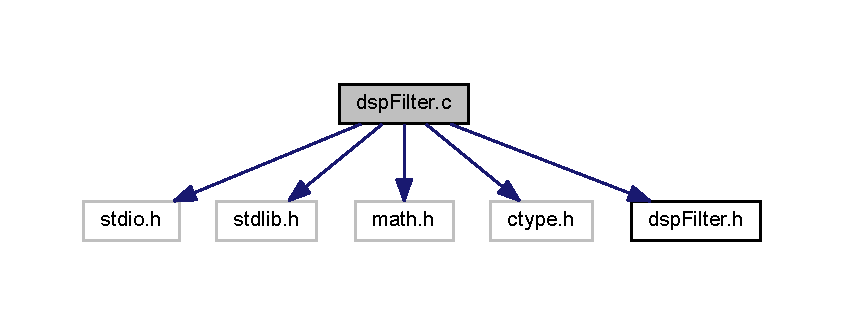
\includegraphics[width=350pt]{d0/d18/dsp_filter_8c__incl}
\end{center}
\end{figure}
\subsection*{함수}
\begin{DoxyCompactItemize}
\item 
void \hyperlink{dsp_filter_8c_a8d5e02bc4a738671a9b7841ea6d12e2c}{Shelving\+Filter2nd\+Low} (\hyperlink{dsp_filter_8h_aeceef54faa278512cd3b46e47d71de18}{\+\_\+\+F\+I\+L\+T\+\_\+\+C\+O\+E\+F} $\ast$param\+\_\+\+Filt\+Coef, float param\+\_\+freq, float param\+\_\+q\+Value, float param\+\_\+gain\+Db)
\begin{DoxyCompactList}\small\item\em 2nd Order Low Frequency Shelving Filter Coefficient Calculation Function \end{DoxyCompactList}\item 
void \hyperlink{dsp_filter_8c_a15386878cb5f5b907f6d2a31f6b275f4}{Shelving\+Filter2nd\+High} (\hyperlink{dsp_filter_8h_aeceef54faa278512cd3b46e47d71de18}{\+\_\+\+F\+I\+L\+T\+\_\+\+C\+O\+E\+F} $\ast$param\+\_\+\+Filt\+Coef, float param\+\_\+freq, float param\+\_\+q\+Value, float param\+\_\+gain\+Db)
\begin{DoxyCompactList}\small\item\em 2nd Order High Frequency Shelving Filter Coefficient Calculation \end{DoxyCompactList}\item 
void \hyperlink{dsp_filter_8c_a254ee3f6745efa5920e091b8a8ef666f}{Peaking\+Filter} (\hyperlink{dsp_filter_8h_aeceef54faa278512cd3b46e47d71de18}{\+\_\+\+F\+I\+L\+T\+\_\+\+C\+O\+E\+F} $\ast$param\+\_\+\+Filt\+Coef, float param\+\_\+freq, float param\+\_\+q\+Value, float param\+\_\+gain\+Db)
\item 
void \hyperlink{dsp_filter_8c_a96bf6847c0943b24c9809daa7fc081a9}{Peq\+Filter} (\hyperlink{dsp_filter_8h_aeceef54faa278512cd3b46e47d71de18}{\+\_\+\+F\+I\+L\+T\+\_\+\+C\+O\+E\+F} $\ast$param\+\_\+\+Filt\+Coef, float param\+\_\+freq, float param\+\_\+q\+Value, float param\+\_\+gain\+Db)
\item 
void \hyperlink{dsp_filter_8c_ae890b45a0c6b9efc1dd5bf146312f21a}{Shelving\+Filter1st\+Low} (\hyperlink{dsp_filter_8h_aeceef54faa278512cd3b46e47d71de18}{\+\_\+\+F\+I\+L\+T\+\_\+\+C\+O\+E\+F} $\ast$param\+\_\+\+Filt\+Coef, float param\+\_\+freq, float param\+\_\+q\+Value, float param\+\_\+gain\+Db)
\end{DoxyCompactItemize}
\subsection*{변수}
\begin{DoxyCompactItemize}
\item 
const float \hyperlink{dsp_filter_8c_ada0744b21abba6961e3e55749e1eee1f}{g\+\_\+two\+Pi}
\item 
const float \hyperlink{dsp_filter_8c_a171eefc2107c2a6148dd6b050aa629ea}{g\+\_\+fs}
\end{DoxyCompactItemize}


\subsection{상세한 설명}
Created on\+: 2015. 6. 10. Author\+: i04055dt 

\hyperlink{dsp_filter_8c_source}{dsp\+Filter.\+c} 파일에서 정의되었습니다.



\subsection{함수 문서화}
\hypertarget{dsp_filter_8c_a254ee3f6745efa5920e091b8a8ef666f}{\index{dsp\+Filter.\+c@{dsp\+Filter.\+c}!Peaking\+Filter@{Peaking\+Filter}}
\index{Peaking\+Filter@{Peaking\+Filter}!dsp\+Filter.\+c@{dsp\+Filter.\+c}}
\subsubsection[{Peaking\+Filter}]{\setlength{\rightskip}{0pt plus 5cm}void Peaking\+Filter (
\begin{DoxyParamCaption}
\item[{{\bf \+\_\+\+F\+I\+L\+T\+\_\+\+C\+O\+E\+F} $\ast$}]{param\+\_\+\+Filt\+Coef, }
\item[{float}]{param\+\_\+freq, }
\item[{float}]{param\+\_\+q\+Value, }
\item[{float}]{param\+\_\+gain\+Db}
\end{DoxyParamCaption}
)}}\label{dsp_filter_8c_a254ee3f6745efa5920e091b8a8ef666f}
2nd Order Peaking Filter Coefficient Calculation Function 
\begin{DoxyParams}{매개변수}
{\em param\+\_\+\+Filt\+Coef} & \\
\hline
{\em param\+\_\+freq} & \\
\hline
{\em param\+\_\+q\+Value} & \\
\hline
{\em param\+\_\+gain\+Db} & \\
\hline
\end{DoxyParams}


dsp\+Filter.\+c 파일의 126 번째 라인에서 정의되었습니다.



다음을 참조함 \+:  \+\_\+\+\_\+\+F\+I\+L\+T\+\_\+\+C\+O\+E\+F\+::a1, \+\_\+\+\_\+\+F\+I\+L\+T\+\_\+\+C\+O\+E\+F\+::a2, \+\_\+\+\_\+\+F\+I\+L\+T\+\_\+\+C\+O\+E\+F\+::b0, \+\_\+\+\_\+\+F\+I\+L\+T\+\_\+\+C\+O\+E\+F\+::b1, \+\_\+\+\_\+\+F\+I\+L\+T\+\_\+\+C\+O\+E\+F\+::b2, g\+\_\+fs, g\+\_\+two\+Pi.

\hypertarget{dsp_filter_8c_a96bf6847c0943b24c9809daa7fc081a9}{\index{dsp\+Filter.\+c@{dsp\+Filter.\+c}!Peq\+Filter@{Peq\+Filter}}
\index{Peq\+Filter@{Peq\+Filter}!dsp\+Filter.\+c@{dsp\+Filter.\+c}}
\subsubsection[{Peq\+Filter}]{\setlength{\rightskip}{0pt plus 5cm}void Peq\+Filter (
\begin{DoxyParamCaption}
\item[{{\bf \+\_\+\+F\+I\+L\+T\+\_\+\+C\+O\+E\+F} $\ast$}]{param\+\_\+\+Filt\+Coef, }
\item[{float}]{param\+\_\+freq, }
\item[{float}]{param\+\_\+q\+Value, }
\item[{float}]{param\+\_\+gain\+Db}
\end{DoxyParamCaption}
)}}\label{dsp_filter_8c_a96bf6847c0943b24c9809daa7fc081a9}
2nd Order Biquad P\+E\+Q Filter Coefficient Calculation Function 
\begin{DoxyParams}{매개변수}
{\em param\+\_\+\+Filt\+Coef} & \\
\hline
{\em param\+\_\+freq} & \\
\hline
{\em param\+\_\+gain\+Db} & \\
\hline
{\em param\+\_\+q\+Value} & \\
\hline
\end{DoxyParams}


dsp\+Filter.\+c 파일의 177 번째 라인에서 정의되었습니다.



다음을 참조함 \+:  \+\_\+\+\_\+\+F\+I\+L\+T\+\_\+\+C\+O\+E\+F\+::a1, \+\_\+\+\_\+\+F\+I\+L\+T\+\_\+\+C\+O\+E\+F\+::a2, \+\_\+\+\_\+\+F\+I\+L\+T\+\_\+\+C\+O\+E\+F\+::b0, \+\_\+\+\_\+\+F\+I\+L\+T\+\_\+\+C\+O\+E\+F\+::b1, \+\_\+\+\_\+\+F\+I\+L\+T\+\_\+\+C\+O\+E\+F\+::b2, g\+\_\+fs, g\+\_\+two\+Pi.

\hypertarget{dsp_filter_8c_ae890b45a0c6b9efc1dd5bf146312f21a}{\index{dsp\+Filter.\+c@{dsp\+Filter.\+c}!Shelving\+Filter1st\+Low@{Shelving\+Filter1st\+Low}}
\index{Shelving\+Filter1st\+Low@{Shelving\+Filter1st\+Low}!dsp\+Filter.\+c@{dsp\+Filter.\+c}}
\subsubsection[{Shelving\+Filter1st\+Low}]{\setlength{\rightskip}{0pt plus 5cm}void Shelving\+Filter1st\+Low (
\begin{DoxyParamCaption}
\item[{{\bf \+\_\+\+F\+I\+L\+T\+\_\+\+C\+O\+E\+F} $\ast$}]{param\+\_\+\+Filt\+Coef, }
\item[{float}]{param\+\_\+freq, }
\item[{float}]{param\+\_\+q\+Value, }
\item[{float}]{param\+\_\+gain\+Db}
\end{DoxyParamCaption}
)}}\label{dsp_filter_8c_ae890b45a0c6b9efc1dd5bf146312f21a}
1st Order Low Frequency Shelving Filter Coefficient Calculation Function 
\begin{DoxyParams}{매개변수}
{\em param\+\_\+\+Filt\+Coef} & \\
\hline
{\em param\+\_\+freq} & \\
\hline
{\em param\+\_\+gain\+Db} & \\
\hline
{\em param\+\_\+q\+Value} & \\
\hline
\end{DoxyParams}


dsp\+Filter.\+c 파일의 242 번째 라인에서 정의되었습니다.



다음을 참조함 \+:  \+\_\+\+\_\+\+F\+I\+L\+T\+\_\+\+C\+O\+E\+F\+::a1, \+\_\+\+\_\+\+F\+I\+L\+T\+\_\+\+C\+O\+E\+F\+::a2, \+\_\+\+\_\+\+F\+I\+L\+T\+\_\+\+C\+O\+E\+F\+::b0, \+\_\+\+\_\+\+F\+I\+L\+T\+\_\+\+C\+O\+E\+F\+::b1, \+\_\+\+\_\+\+F\+I\+L\+T\+\_\+\+C\+O\+E\+F\+::b2, g\+\_\+fs, g\+\_\+two\+Pi.

\hypertarget{dsp_filter_8c_a15386878cb5f5b907f6d2a31f6b275f4}{\index{dsp\+Filter.\+c@{dsp\+Filter.\+c}!Shelving\+Filter2nd\+High@{Shelving\+Filter2nd\+High}}
\index{Shelving\+Filter2nd\+High@{Shelving\+Filter2nd\+High}!dsp\+Filter.\+c@{dsp\+Filter.\+c}}
\subsubsection[{Shelving\+Filter2nd\+High}]{\setlength{\rightskip}{0pt plus 5cm}void Shelving\+Filter2nd\+High (
\begin{DoxyParamCaption}
\item[{{\bf \+\_\+\+F\+I\+L\+T\+\_\+\+C\+O\+E\+F} $\ast$}]{param\+\_\+\+Filt\+Coef, }
\item[{float}]{param\+\_\+freq, }
\item[{float}]{param\+\_\+q\+Value, }
\item[{float}]{param\+\_\+gain\+Db}
\end{DoxyParamCaption}
)}}\label{dsp_filter_8c_a15386878cb5f5b907f6d2a31f6b275f4}


2nd Order High Frequency Shelving Filter Coefficient Calculation 


\begin{DoxyParams}{매개변수}
{\em param\+\_\+\+Filt\+Coef} & \\
\hline
{\em param\+\_\+freq} & \\
\hline
{\em param\+\_\+gain\+Db} & \\
\hline
{\em param\+\_\+q\+Value} & \\
\hline
\end{DoxyParams}


dsp\+Filter.\+c 파일의 76 번째 라인에서 정의되었습니다.



다음을 참조함 \+:  \+\_\+\+\_\+\+F\+I\+L\+T\+\_\+\+C\+O\+E\+F\+::a1, \+\_\+\+\_\+\+F\+I\+L\+T\+\_\+\+C\+O\+E\+F\+::a2, \+\_\+\+\_\+\+F\+I\+L\+T\+\_\+\+C\+O\+E\+F\+::b0, \+\_\+\+\_\+\+F\+I\+L\+T\+\_\+\+C\+O\+E\+F\+::b1, \+\_\+\+\_\+\+F\+I\+L\+T\+\_\+\+C\+O\+E\+F\+::b2, g\+\_\+fs, g\+\_\+two\+Pi.

\hypertarget{dsp_filter_8c_a8d5e02bc4a738671a9b7841ea6d12e2c}{\index{dsp\+Filter.\+c@{dsp\+Filter.\+c}!Shelving\+Filter2nd\+Low@{Shelving\+Filter2nd\+Low}}
\index{Shelving\+Filter2nd\+Low@{Shelving\+Filter2nd\+Low}!dsp\+Filter.\+c@{dsp\+Filter.\+c}}
\subsubsection[{Shelving\+Filter2nd\+Low}]{\setlength{\rightskip}{0pt plus 5cm}void Shelving\+Filter2nd\+Low (
\begin{DoxyParamCaption}
\item[{{\bf \+\_\+\+F\+I\+L\+T\+\_\+\+C\+O\+E\+F} $\ast$}]{param\+\_\+\+Filt\+Coef, }
\item[{float}]{param\+\_\+freq, }
\item[{float}]{param\+\_\+q\+Value, }
\item[{float}]{param\+\_\+gain\+Db}
\end{DoxyParamCaption}
)}}\label{dsp_filter_8c_a8d5e02bc4a738671a9b7841ea6d12e2c}


2nd Order Low Frequency Shelving Filter Coefficient Calculation Function 


\begin{DoxyParams}{매개변수}
{\em param\+\_\+\+Filt\+Coef} & \\
\hline
{\em param\+\_\+freq} & \\
\hline
{\em param\+\_\+q\+Value} & \\
\hline
{\em param\+\_\+gain\+Db} & \\
\hline
\end{DoxyParams}


dsp\+Filter.\+c 파일의 25 번째 라인에서 정의되었습니다.



다음을 참조함 \+:  \+\_\+\+\_\+\+F\+I\+L\+T\+\_\+\+C\+O\+E\+F\+::a1, \+\_\+\+\_\+\+F\+I\+L\+T\+\_\+\+C\+O\+E\+F\+::a2, \+\_\+\+\_\+\+F\+I\+L\+T\+\_\+\+C\+O\+E\+F\+::b0, \+\_\+\+\_\+\+F\+I\+L\+T\+\_\+\+C\+O\+E\+F\+::b1, \+\_\+\+\_\+\+F\+I\+L\+T\+\_\+\+C\+O\+E\+F\+::b2, g\+\_\+fs, g\+\_\+two\+Pi.



\subsection{변수 문서화}
\hypertarget{dsp_filter_8c_a171eefc2107c2a6148dd6b050aa629ea}{\index{dsp\+Filter.\+c@{dsp\+Filter.\+c}!g\+\_\+fs@{g\+\_\+fs}}
\index{g\+\_\+fs@{g\+\_\+fs}!dsp\+Filter.\+c@{dsp\+Filter.\+c}}
\subsubsection[{g\+\_\+fs}]{\setlength{\rightskip}{0pt plus 5cm}const float g\+\_\+fs}}\label{dsp_filter_8c_a171eefc2107c2a6148dd6b050aa629ea}


dsp\+Q\+Format\+Convert.\+c 파일의 15 번째 라인에서 정의되었습니다.



다음에 의해서 참조됨 \+:  Peaking\+Filter(), Peq\+Filter(), Shelving\+Filter1st\+Low(), Shelving\+Filter2nd\+High(), Shelving\+Filter2nd\+Low().

\hypertarget{dsp_filter_8c_ada0744b21abba6961e3e55749e1eee1f}{\index{dsp\+Filter.\+c@{dsp\+Filter.\+c}!g\+\_\+two\+Pi@{g\+\_\+two\+Pi}}
\index{g\+\_\+two\+Pi@{g\+\_\+two\+Pi}!dsp\+Filter.\+c@{dsp\+Filter.\+c}}
\subsubsection[{g\+\_\+two\+Pi}]{\setlength{\rightskip}{0pt plus 5cm}const float g\+\_\+two\+Pi}}\label{dsp_filter_8c_ada0744b21abba6961e3e55749e1eee1f}


dsp\+Q\+Format\+Convert.\+c 파일의 14 번째 라인에서 정의되었습니다.



다음에 의해서 참조됨 \+:  Peaking\+Filter(), Peq\+Filter(), Shelving\+Filter1st\+Low(), Shelving\+Filter2nd\+High(), Shelving\+Filter2nd\+Low().


\hypertarget{dsp_filter_8h}{\section{dsp\+Filter.\+h 파일 참조}
\label{dsp_filter_8h}\index{dsp\+Filter.\+h@{dsp\+Filter.\+h}}
}
이 그래프는 이 파일을 직/간접적으로 include 하는 파일들을 보여줍니다.\+:
\nopagebreak
\begin{figure}[H]
\begin{center}
\leavevmode
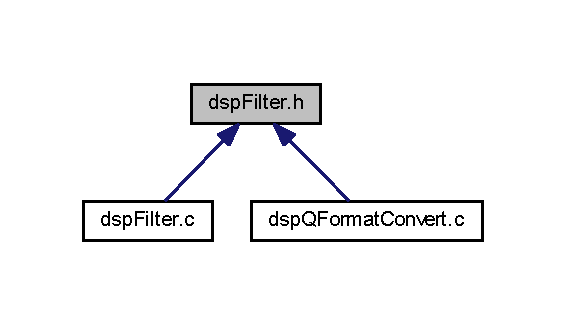
\includegraphics[width=272pt]{de/d37/dsp_filter_8h__dep__incl}
\end{center}
\end{figure}
\subsection*{데이타 구조}
\begin{DoxyCompactItemize}
\item 
struct \hyperlink{struct_____f_i_l_t___c_o_e_f}{\+\_\+\+\_\+\+F\+I\+L\+T\+\_\+\+C\+O\+E\+F}
\begin{DoxyCompactList}\small\item\em Floating point Filter Coefficient Structures. \end{DoxyCompactList}\item 
struct \hyperlink{struct_____q___f_o_r_m_a_t}{\+\_\+\+\_\+\+Q\+\_\+\+F\+O\+R\+M\+A\+T}
\begin{DoxyCompactList}\small\item\em Q Formatted Filter Coefficient Sturctures. \end{DoxyCompactList}\end{DoxyCompactItemize}
\subsection*{타입정의}
\begin{DoxyCompactItemize}
\item 
typedef struct \hyperlink{struct_____f_i_l_t___c_o_e_f}{\+\_\+\+\_\+\+F\+I\+L\+T\+\_\+\+C\+O\+E\+F} \hyperlink{dsp_filter_8h_aeceef54faa278512cd3b46e47d71de18}{\+\_\+\+F\+I\+L\+T\+\_\+\+C\+O\+E\+F}
\begin{DoxyCompactList}\small\item\em Floating point Filter Coefficient Structures. \end{DoxyCompactList}\item 
typedef struct \hyperlink{struct_____q___f_o_r_m_a_t}{\+\_\+\+\_\+\+Q\+\_\+\+F\+O\+R\+M\+A\+T} \hyperlink{dsp_filter_8h_ad441c1c66a421036640642bf5f66b7fa}{\+\_\+\+Q\+\_\+\+F\+O\+R\+M\+A\+T}
\begin{DoxyCompactList}\small\item\em Q Formatted Filter Coefficient Sturctures. \end{DoxyCompactList}\end{DoxyCompactItemize}
\subsection*{함수}
\begin{DoxyCompactItemize}
\item 
void \hyperlink{dsp_filter_8h_a8d5e02bc4a738671a9b7841ea6d12e2c}{Shelving\+Filter2nd\+Low} (\hyperlink{dsp_filter_8h_aeceef54faa278512cd3b46e47d71de18}{\+\_\+\+F\+I\+L\+T\+\_\+\+C\+O\+E\+F} $\ast$param\+\_\+\+Filt\+Coef, float param\+\_\+freq, float param\+\_\+q\+Value, float param\+\_\+gain\+Db)
\begin{DoxyCompactList}\small\item\em 2nd Order Low Frequency Shelving Filter Coefficient Calculation Function \end{DoxyCompactList}\item 
void \hyperlink{dsp_filter_8h_a15386878cb5f5b907f6d2a31f6b275f4}{Shelving\+Filter2nd\+High} (\hyperlink{dsp_filter_8h_aeceef54faa278512cd3b46e47d71de18}{\+\_\+\+F\+I\+L\+T\+\_\+\+C\+O\+E\+F} $\ast$param\+\_\+\+Filt\+Coef, float param\+\_\+freq, float param\+\_\+q\+Value, float param\+\_\+gain\+Db)
\begin{DoxyCompactList}\small\item\em 2nd Order High Frequency Shelving Filter Coefficient Calculation \end{DoxyCompactList}\item 
void \hyperlink{dsp_filter_8h_a254ee3f6745efa5920e091b8a8ef666f}{Peaking\+Filter} (\hyperlink{dsp_filter_8h_aeceef54faa278512cd3b46e47d71de18}{\+\_\+\+F\+I\+L\+T\+\_\+\+C\+O\+E\+F} $\ast$param\+\_\+\+Filt\+Coef, float param\+\_\+freq, float param\+\_\+q\+Value, float param\+\_\+gain\+Db)
\item 
void \hyperlink{dsp_filter_8h_a96bf6847c0943b24c9809daa7fc081a9}{Peq\+Filter} (\hyperlink{dsp_filter_8h_aeceef54faa278512cd3b46e47d71de18}{\+\_\+\+F\+I\+L\+T\+\_\+\+C\+O\+E\+F} $\ast$param\+\_\+\+Filt\+Coef, float param\+\_\+freq, float param\+\_\+q\+Value, float param\+\_\+gain\+Db)
\item 
void \hyperlink{dsp_filter_8h_ae890b45a0c6b9efc1dd5bf146312f21a}{Shelving\+Filter1st\+Low} (\hyperlink{dsp_filter_8h_aeceef54faa278512cd3b46e47d71de18}{\+\_\+\+F\+I\+L\+T\+\_\+\+C\+O\+E\+F} $\ast$param\+\_\+\+Filt\+Coef, float param\+\_\+freq, float param\+\_\+q\+Value, float param\+\_\+gain\+Db)
\end{DoxyCompactItemize}


\subsection{타입정의 문서화}
\hypertarget{dsp_filter_8h_aeceef54faa278512cd3b46e47d71de18}{\index{dsp\+Filter.\+h@{dsp\+Filter.\+h}!\+\_\+\+F\+I\+L\+T\+\_\+\+C\+O\+E\+F@{\+\_\+\+F\+I\+L\+T\+\_\+\+C\+O\+E\+F}}
\index{\+\_\+\+F\+I\+L\+T\+\_\+\+C\+O\+E\+F@{\+\_\+\+F\+I\+L\+T\+\_\+\+C\+O\+E\+F}!dsp\+Filter.\+h@{dsp\+Filter.\+h}}
\subsubsection[{\+\_\+\+F\+I\+L\+T\+\_\+\+C\+O\+E\+F}]{\setlength{\rightskip}{0pt plus 5cm}typedef struct {\bf \+\_\+\+\_\+\+F\+I\+L\+T\+\_\+\+C\+O\+E\+F}  {\bf \+\_\+\+F\+I\+L\+T\+\_\+\+C\+O\+E\+F}}}\label{dsp_filter_8h_aeceef54faa278512cd3b46e47d71de18}


Floating point Filter Coefficient Structures. 

\hyperlink{dsp_filter_8h}{dsp\+Filter.\+h}

Created on\+: 2015. 6. 10. Author\+: i04055dt \hypertarget{dsp_filter_8h_ad441c1c66a421036640642bf5f66b7fa}{\index{dsp\+Filter.\+h@{dsp\+Filter.\+h}!\+\_\+\+Q\+\_\+\+F\+O\+R\+M\+A\+T@{\+\_\+\+Q\+\_\+\+F\+O\+R\+M\+A\+T}}
\index{\+\_\+\+Q\+\_\+\+F\+O\+R\+M\+A\+T@{\+\_\+\+Q\+\_\+\+F\+O\+R\+M\+A\+T}!dsp\+Filter.\+h@{dsp\+Filter.\+h}}
\subsubsection[{\+\_\+\+Q\+\_\+\+F\+O\+R\+M\+A\+T}]{\setlength{\rightskip}{0pt plus 5cm}typedef struct {\bf \+\_\+\+\_\+\+Q\+\_\+\+F\+O\+R\+M\+A\+T}  {\bf \+\_\+\+Q\+\_\+\+F\+O\+R\+M\+A\+T}}}\label{dsp_filter_8h_ad441c1c66a421036640642bf5f66b7fa}


Q Formatted Filter Coefficient Sturctures. 



\subsection{함수 문서화}
\hypertarget{dsp_filter_8h_a254ee3f6745efa5920e091b8a8ef666f}{\index{dsp\+Filter.\+h@{dsp\+Filter.\+h}!Peaking\+Filter@{Peaking\+Filter}}
\index{Peaking\+Filter@{Peaking\+Filter}!dsp\+Filter.\+h@{dsp\+Filter.\+h}}
\subsubsection[{Peaking\+Filter}]{\setlength{\rightskip}{0pt plus 5cm}void Peaking\+Filter (
\begin{DoxyParamCaption}
\item[{{\bf \+\_\+\+F\+I\+L\+T\+\_\+\+C\+O\+E\+F} $\ast$}]{param\+\_\+\+Filt\+Coef, }
\item[{float}]{param\+\_\+freq, }
\item[{float}]{param\+\_\+q\+Value, }
\item[{float}]{param\+\_\+gain\+Db}
\end{DoxyParamCaption}
)}}\label{dsp_filter_8h_a254ee3f6745efa5920e091b8a8ef666f}
2nd Order Peaking Filter Coefficient Calculation Function 
\begin{DoxyParams}{매개변수}
{\em param\+\_\+\+Filt\+Coef} & \\
\hline
{\em param\+\_\+freq} & \\
\hline
{\em param\+\_\+q\+Value} & \\
\hline
{\em param\+\_\+gain\+Db} & \\
\hline
\end{DoxyParams}


dsp\+Filter.\+c 파일의 126 번째 라인에서 정의되었습니다.



다음을 참조함 \+:  \+\_\+\+\_\+\+F\+I\+L\+T\+\_\+\+C\+O\+E\+F\+::a1, \+\_\+\+\_\+\+F\+I\+L\+T\+\_\+\+C\+O\+E\+F\+::a2, \+\_\+\+\_\+\+F\+I\+L\+T\+\_\+\+C\+O\+E\+F\+::b0, \+\_\+\+\_\+\+F\+I\+L\+T\+\_\+\+C\+O\+E\+F\+::b1, \+\_\+\+\_\+\+F\+I\+L\+T\+\_\+\+C\+O\+E\+F\+::b2, g\+\_\+fs, g\+\_\+two\+Pi.

\hypertarget{dsp_filter_8h_a96bf6847c0943b24c9809daa7fc081a9}{\index{dsp\+Filter.\+h@{dsp\+Filter.\+h}!Peq\+Filter@{Peq\+Filter}}
\index{Peq\+Filter@{Peq\+Filter}!dsp\+Filter.\+h@{dsp\+Filter.\+h}}
\subsubsection[{Peq\+Filter}]{\setlength{\rightskip}{0pt plus 5cm}void Peq\+Filter (
\begin{DoxyParamCaption}
\item[{{\bf \+\_\+\+F\+I\+L\+T\+\_\+\+C\+O\+E\+F} $\ast$}]{param\+\_\+\+Filt\+Coef, }
\item[{float}]{param\+\_\+freq, }
\item[{float}]{param\+\_\+q\+Value, }
\item[{float}]{param\+\_\+gain\+Db}
\end{DoxyParamCaption}
)}}\label{dsp_filter_8h_a96bf6847c0943b24c9809daa7fc081a9}
2nd Order Biquad P\+E\+Q Filter Coefficient Calculation Function 
\begin{DoxyParams}{매개변수}
{\em param\+\_\+\+Filt\+Coef} & \\
\hline
{\em param\+\_\+freq} & \\
\hline
{\em param\+\_\+gain\+Db} & \\
\hline
{\em param\+\_\+q\+Value} & \\
\hline
\end{DoxyParams}


dsp\+Filter.\+c 파일의 177 번째 라인에서 정의되었습니다.



다음을 참조함 \+:  \+\_\+\+\_\+\+F\+I\+L\+T\+\_\+\+C\+O\+E\+F\+::a1, \+\_\+\+\_\+\+F\+I\+L\+T\+\_\+\+C\+O\+E\+F\+::a2, \+\_\+\+\_\+\+F\+I\+L\+T\+\_\+\+C\+O\+E\+F\+::b0, \+\_\+\+\_\+\+F\+I\+L\+T\+\_\+\+C\+O\+E\+F\+::b1, \+\_\+\+\_\+\+F\+I\+L\+T\+\_\+\+C\+O\+E\+F\+::b2, g\+\_\+fs, g\+\_\+two\+Pi.

\hypertarget{dsp_filter_8h_ae890b45a0c6b9efc1dd5bf146312f21a}{\index{dsp\+Filter.\+h@{dsp\+Filter.\+h}!Shelving\+Filter1st\+Low@{Shelving\+Filter1st\+Low}}
\index{Shelving\+Filter1st\+Low@{Shelving\+Filter1st\+Low}!dsp\+Filter.\+h@{dsp\+Filter.\+h}}
\subsubsection[{Shelving\+Filter1st\+Low}]{\setlength{\rightskip}{0pt plus 5cm}void Shelving\+Filter1st\+Low (
\begin{DoxyParamCaption}
\item[{{\bf \+\_\+\+F\+I\+L\+T\+\_\+\+C\+O\+E\+F} $\ast$}]{param\+\_\+\+Filt\+Coef, }
\item[{float}]{param\+\_\+freq, }
\item[{float}]{param\+\_\+q\+Value, }
\item[{float}]{param\+\_\+gain\+Db}
\end{DoxyParamCaption}
)}}\label{dsp_filter_8h_ae890b45a0c6b9efc1dd5bf146312f21a}
1st Order Low Frequency Shelving Filter Coefficient Calculation Function 
\begin{DoxyParams}{매개변수}
{\em param\+\_\+\+Filt\+Coef} & \\
\hline
{\em param\+\_\+freq} & \\
\hline
{\em param\+\_\+gain\+Db} & \\
\hline
{\em param\+\_\+q\+Value} & \\
\hline
\end{DoxyParams}


dsp\+Filter.\+c 파일의 242 번째 라인에서 정의되었습니다.



다음을 참조함 \+:  \+\_\+\+\_\+\+F\+I\+L\+T\+\_\+\+C\+O\+E\+F\+::a1, \+\_\+\+\_\+\+F\+I\+L\+T\+\_\+\+C\+O\+E\+F\+::a2, \+\_\+\+\_\+\+F\+I\+L\+T\+\_\+\+C\+O\+E\+F\+::b0, \+\_\+\+\_\+\+F\+I\+L\+T\+\_\+\+C\+O\+E\+F\+::b1, \+\_\+\+\_\+\+F\+I\+L\+T\+\_\+\+C\+O\+E\+F\+::b2, g\+\_\+fs, g\+\_\+two\+Pi.

\hypertarget{dsp_filter_8h_a15386878cb5f5b907f6d2a31f6b275f4}{\index{dsp\+Filter.\+h@{dsp\+Filter.\+h}!Shelving\+Filter2nd\+High@{Shelving\+Filter2nd\+High}}
\index{Shelving\+Filter2nd\+High@{Shelving\+Filter2nd\+High}!dsp\+Filter.\+h@{dsp\+Filter.\+h}}
\subsubsection[{Shelving\+Filter2nd\+High}]{\setlength{\rightskip}{0pt plus 5cm}void Shelving\+Filter2nd\+High (
\begin{DoxyParamCaption}
\item[{{\bf \+\_\+\+F\+I\+L\+T\+\_\+\+C\+O\+E\+F} $\ast$}]{param\+\_\+\+Filt\+Coef, }
\item[{float}]{param\+\_\+freq, }
\item[{float}]{param\+\_\+q\+Value, }
\item[{float}]{param\+\_\+gain\+Db}
\end{DoxyParamCaption}
)}}\label{dsp_filter_8h_a15386878cb5f5b907f6d2a31f6b275f4}


2nd Order High Frequency Shelving Filter Coefficient Calculation 


\begin{DoxyParams}{매개변수}
{\em param\+\_\+\+Filt\+Coef} & \\
\hline
{\em param\+\_\+freq} & \\
\hline
{\em param\+\_\+gain\+Db} & \\
\hline
{\em param\+\_\+q\+Value} & \\
\hline
\end{DoxyParams}


dsp\+Filter.\+c 파일의 76 번째 라인에서 정의되었습니다.



다음을 참조함 \+:  \+\_\+\+\_\+\+F\+I\+L\+T\+\_\+\+C\+O\+E\+F\+::a1, \+\_\+\+\_\+\+F\+I\+L\+T\+\_\+\+C\+O\+E\+F\+::a2, \+\_\+\+\_\+\+F\+I\+L\+T\+\_\+\+C\+O\+E\+F\+::b0, \+\_\+\+\_\+\+F\+I\+L\+T\+\_\+\+C\+O\+E\+F\+::b1, \+\_\+\+\_\+\+F\+I\+L\+T\+\_\+\+C\+O\+E\+F\+::b2, g\+\_\+fs, g\+\_\+two\+Pi.

\hypertarget{dsp_filter_8h_a8d5e02bc4a738671a9b7841ea6d12e2c}{\index{dsp\+Filter.\+h@{dsp\+Filter.\+h}!Shelving\+Filter2nd\+Low@{Shelving\+Filter2nd\+Low}}
\index{Shelving\+Filter2nd\+Low@{Shelving\+Filter2nd\+Low}!dsp\+Filter.\+h@{dsp\+Filter.\+h}}
\subsubsection[{Shelving\+Filter2nd\+Low}]{\setlength{\rightskip}{0pt plus 5cm}void Shelving\+Filter2nd\+Low (
\begin{DoxyParamCaption}
\item[{{\bf \+\_\+\+F\+I\+L\+T\+\_\+\+C\+O\+E\+F} $\ast$}]{param\+\_\+\+Filt\+Coef, }
\item[{float}]{param\+\_\+freq, }
\item[{float}]{param\+\_\+q\+Value, }
\item[{float}]{param\+\_\+gain\+Db}
\end{DoxyParamCaption}
)}}\label{dsp_filter_8h_a8d5e02bc4a738671a9b7841ea6d12e2c}


2nd Order Low Frequency Shelving Filter Coefficient Calculation Function 


\begin{DoxyParams}{매개변수}
{\em param\+\_\+\+Filt\+Coef} & \\
\hline
{\em param\+\_\+freq} & \\
\hline
{\em param\+\_\+q\+Value} & \\
\hline
{\em param\+\_\+gain\+Db} & \\
\hline
\end{DoxyParams}


dsp\+Filter.\+c 파일의 25 번째 라인에서 정의되었습니다.



다음을 참조함 \+:  \+\_\+\+\_\+\+F\+I\+L\+T\+\_\+\+C\+O\+E\+F\+::a1, \+\_\+\+\_\+\+F\+I\+L\+T\+\_\+\+C\+O\+E\+F\+::a2, \+\_\+\+\_\+\+F\+I\+L\+T\+\_\+\+C\+O\+E\+F\+::b0, \+\_\+\+\_\+\+F\+I\+L\+T\+\_\+\+C\+O\+E\+F\+::b1, \+\_\+\+\_\+\+F\+I\+L\+T\+\_\+\+C\+O\+E\+F\+::b2, g\+\_\+fs, g\+\_\+two\+Pi.


\hypertarget{dsp_q_format_convert_8c}{\section{dsp\+Q\+Format\+Convert.\+c 파일 참조}
\label{dsp_q_format_convert_8c}\index{dsp\+Q\+Format\+Convert.\+c@{dsp\+Q\+Format\+Convert.\+c}}
}
{\ttfamily \#include $<$stdio.\+h$>$}\\*
{\ttfamily \#include $<$stdlib.\+h$>$}\\*
{\ttfamily \#include $<$math.\+h$>$}\\*
{\ttfamily \#include \char`\"{}dsp\+Filter.\+h\char`\"{}}\\*
{\ttfamily \#include \char`\"{}dsp\+Q\+Format\+Convert.\+h\char`\"{}}\\*
dsp\+Q\+Format\+Convert.\+c에 대한 include 의존 그래프
\nopagebreak
\begin{figure}[H]
\begin{center}
\leavevmode
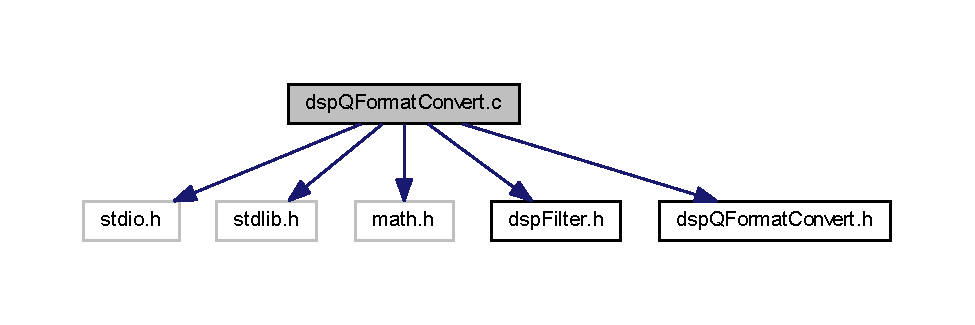
\includegraphics[width=350pt]{d5/d43/dsp_q_format_convert_8c__incl}
\end{center}
\end{figure}
\subsection*{함수}
\begin{DoxyCompactItemize}
\item 
int \hyperlink{dsp_q_format_convert_8c_a646289654152ae05600606013b945c86}{Float2\+Q\+Format\+Convert} (\hyperlink{dsp_filter_8h_aeceef54faa278512cd3b46e47d71de18}{\+\_\+\+F\+I\+L\+T\+\_\+\+C\+O\+E\+F} param\+\_\+t\+Filt\+Coef, \hyperlink{dsp_filter_8h_ad441c1c66a421036640642bf5f66b7fa}{\+\_\+\+Q\+\_\+\+F\+O\+R\+M\+A\+T} $\ast$param\+\_\+t\+Filt\+Q\+Form, unsigned int fix\+Num, unsigned int frac\+Num)
\begin{DoxyCompactList}\small\item\em Floating Point Filter Coefficient convert to Fixed Point Q Format Qm.\+n~\newline
. \end{DoxyCompactList}\item 
int \hyperlink{dsp_q_format_convert_8c_afdb499fad2e27d0ac12c8ff37876f234}{Q\+Format2\+Float\+Convert} (\hyperlink{dsp_filter_8h_ad441c1c66a421036640642bf5f66b7fa}{\+\_\+\+Q\+\_\+\+F\+O\+R\+M\+A\+T} param\+\_\+filt\+Q\+Form, \hyperlink{dsp_filter_8h_aeceef54faa278512cd3b46e47d71de18}{\+\_\+\+F\+I\+L\+T\+\_\+\+C\+O\+E\+F} $\ast$param\+\_\+filt\+Coef, unsigned int fix\+Num, unsigned int frac\+Num)
\item 
void \hyperlink{dsp_q_format_convert_8c_a5f03ce0a0de11a675df423d641fe58b2}{Print\+Coef} (int mode, \hyperlink{dsp_filter_8h_aeceef54faa278512cd3b46e47d71de18}{\+\_\+\+F\+I\+L\+T\+\_\+\+C\+O\+E\+F} param\+\_\+t\+Filt\+Coef, \hyperlink{dsp_filter_8h_ad441c1c66a421036640642bf5f66b7fa}{\+\_\+\+Q\+\_\+\+F\+O\+R\+M\+A\+T} param\+\_\+t\+Filt\+Q\+Form, float val\+Freq, float val\+Q, float val\+Gain)
\item 
int \hyperlink{dsp_q_format_convert_8c_a16501f69f57199c5dc647b0fdb9f00bb}{Q\+Format\+Convert} (float param\+\_\+filt\+Coef, int $\ast$param\+\_\+filt\+Q\+Form, unsigned int frac\+Num)
\begin{DoxyCompactList}\small\item\em Q Format Converter Function. \end{DoxyCompactList}\item 
int \hyperlink{dsp_q_format_convert_8c_a81334f577bbbfde46b471108f5a648d4}{Q\+Form2\+Float\+Converter} (int param\+\_\+filt\+Q\+Form, float $\ast$param\+\_\+filt\+Coef, unsigned int frac\+Num)
\end{DoxyCompactItemize}
\subsection*{변수}
\begin{DoxyCompactItemize}
\item 
const float \hyperlink{dsp_q_format_convert_8c_ada0744b21abba6961e3e55749e1eee1f}{g\+\_\+two\+Pi} = 6.\+283185307179586476925286766559
\item 
const float \hyperlink{dsp_q_format_convert_8c_a171eefc2107c2a6148dd6b050aa629ea}{g\+\_\+fs} = \hyperlink{dsp_q_format_convert_8h_a4b76a0c2859cfd819a343a780070ee2b}{S\+A\+M\+P\+L\+E\+\_\+\+R\+A\+T\+E}
\item 
const unsigned char \hyperlink{dsp_q_format_convert_8c_a3d43538ea1ab2e5c29aee81a46293698}{str2nd\+Lo\+Shelf\+Filter} \mbox{[}$\,$\mbox{]} = \char`\"{}2nd Order Low Shelf Filter\+:\textbackslash{}0\char`\"{}
\item 
const unsigned char \hyperlink{dsp_q_format_convert_8c_addaa4776cfc6bc81f7fd3bdbc53c48fb}{str2nd\+Hi\+Shelf\+Filter} \mbox{[}$\,$\mbox{]} = \char`\"{}2nd Order High Shelf Filter\+:\textbackslash{}0\char`\"{}
\item 
const unsigned char \hyperlink{dsp_q_format_convert_8c_af1412449d6875a0a2a272e2affa062a9}{str\+Peak\+Filter} \mbox{[}$\,$\mbox{]} = \char`\"{}Peaking Filter\+:\textbackslash{}0\char`\"{}
\item 
const unsigned char \hyperlink{dsp_q_format_convert_8c_a82f69c2969fbcf32622f497a3c348f61}{str\+Peq\+Filter} \mbox{[}$\,$\mbox{]} = \char`\"{}Parametric E\+Q Filter\+:\textbackslash{}0\char`\"{}
\item 
const unsigned char \hyperlink{dsp_q_format_convert_8c_a926c3674b0a07cbef1693833c86098a6}{str1st\+Lo\+Shelf\+Filter} \mbox{[}$\,$\mbox{]} = \char`\"{}1st Order Low Shelf Filter\+:\textbackslash{}0\char`\"{}
\end{DoxyCompactItemize}


\subsection{상세한 설명}
\begin{DoxyDate}{날짜}
2015. 6. 10. 
\end{DoxyDate}
\begin{DoxyAuthor}{작성자}
i04055dt 
\end{DoxyAuthor}


\hyperlink{dsp_q_format_convert_8c_source}{dsp\+Q\+Format\+Convert.\+c} 파일에서 정의되었습니다.



\subsection{함수 문서화}
\hypertarget{dsp_q_format_convert_8c_a646289654152ae05600606013b945c86}{\index{dsp\+Q\+Format\+Convert.\+c@{dsp\+Q\+Format\+Convert.\+c}!Float2\+Q\+Format\+Convert@{Float2\+Q\+Format\+Convert}}
\index{Float2\+Q\+Format\+Convert@{Float2\+Q\+Format\+Convert}!dsp\+Q\+Format\+Convert.\+c@{dsp\+Q\+Format\+Convert.\+c}}
\subsubsection[{Float2\+Q\+Format\+Convert}]{\setlength{\rightskip}{0pt plus 5cm}int Float2\+Q\+Format\+Convert (
\begin{DoxyParamCaption}
\item[{{\bf \+\_\+\+F\+I\+L\+T\+\_\+\+C\+O\+E\+F}}]{param\+\_\+t\+Filt\+Coef, }
\item[{{\bf \+\_\+\+Q\+\_\+\+F\+O\+R\+M\+A\+T} $\ast$}]{param\+\_\+t\+Filt\+Q\+Form, }
\item[{unsigned int}]{fix\+Num, }
\item[{unsigned int}]{frac\+Num}
\end{DoxyParamCaption}
)}}\label{dsp_q_format_convert_8c_a646289654152ae05600606013b945c86}


Floating Point Filter Coefficient convert to Fixed Point Q Format Qm.\+n~\newline
. 


\begin{DoxyItemize}
\item Input/\+Output is the Structure of Filter Coefficients \& Q Format Coefficients
\end{DoxyItemize}


\begin{DoxyParams}{매개변수}
{\em param\+\_\+t\+Filt\+Coef} & Src\+: Floating Point Filter Coefficient \\
\hline
{\em param\+\_\+t\+Filt\+Q\+Form} & Des\+: Q Format Integer Filter Coefficient \\
\hline
{\em fix\+Num} & Q Format Fixed Bit Number \\
\hline
{\em frac\+Num} & Q Format Fraction Bit Number \\
\hline
\end{DoxyParams}
\begin{DoxyReturn}{반환값}
No Error\+: 0, Error\+: -\/1 
\end{DoxyReturn}


dsp\+Q\+Format\+Convert.\+c 파일의 33 번째 라인에서 정의되었습니다.



다음을 참조함 \+:  \+\_\+\+\_\+\+F\+I\+L\+T\+\_\+\+C\+O\+E\+F\+::a1, \+\_\+\+\_\+\+Q\+\_\+\+F\+O\+R\+M\+A\+T\+::a1, \+\_\+\+\_\+\+F\+I\+L\+T\+\_\+\+C\+O\+E\+F\+::a2, \+\_\+\+\_\+\+Q\+\_\+\+F\+O\+R\+M\+A\+T\+::a2, \+\_\+\+\_\+\+F\+I\+L\+T\+\_\+\+C\+O\+E\+F\+::b0, \+\_\+\+\_\+\+Q\+\_\+\+F\+O\+R\+M\+A\+T\+::b0, \+\_\+\+\_\+\+F\+I\+L\+T\+\_\+\+C\+O\+E\+F\+::b1, \+\_\+\+\_\+\+Q\+\_\+\+F\+O\+R\+M\+A\+T\+::b1, \+\_\+\+\_\+\+F\+I\+L\+T\+\_\+\+C\+O\+E\+F\+::b2, \+\_\+\+\_\+\+Q\+\_\+\+F\+O\+R\+M\+A\+T\+::b2.

\hypertarget{dsp_q_format_convert_8c_a5f03ce0a0de11a675df423d641fe58b2}{\index{dsp\+Q\+Format\+Convert.\+c@{dsp\+Q\+Format\+Convert.\+c}!Print\+Coef@{Print\+Coef}}
\index{Print\+Coef@{Print\+Coef}!dsp\+Q\+Format\+Convert.\+c@{dsp\+Q\+Format\+Convert.\+c}}
\subsubsection[{Print\+Coef}]{\setlength{\rightskip}{0pt plus 5cm}void Print\+Coef (
\begin{DoxyParamCaption}
\item[{int}]{mode, }
\item[{{\bf \+\_\+\+F\+I\+L\+T\+\_\+\+C\+O\+E\+F}}]{param\+\_\+t\+Filt\+Coef, }
\item[{{\bf \+\_\+\+Q\+\_\+\+F\+O\+R\+M\+A\+T}}]{param\+\_\+t\+Filt\+Q\+Form, }
\item[{float}]{val\+Freq, }
\item[{float}]{val\+Q, }
\item[{float}]{val\+Gain}
\end{DoxyParamCaption}
)}}\label{dsp_q_format_convert_8c_a5f03ce0a0de11a675df423d641fe58b2}
Print Filter Coefficient Floating Value And Q1.\+31 Format 
\begin{DoxyParams}{매개변수}
{\em mode} & E\+Q Filter Mode~\newline

\begin{DoxyItemize}
\item 0\+: Low Pass Shelving Filter~\newline

\item 1\+: High Pass Shelving Filter~\newline

\item 2\+: Peak Filter~\newline

\item 3\+: Parametric E\+Q Filter~\newline

\item 4\+: 1st order Low Pass Shelving Filter 
\end{DoxyItemize}\\
\hline
{\em param\+\_\+t\+Filt\+Coef} & \\
\hline
{\em param\+\_\+t\+Filt\+Q\+Form} & \\
\hline
{\em val\+Freq} & \\
\hline
{\em val\+Q} & \\
\hline
{\em val\+Gain} & \\
\hline
\end{DoxyParams}


dsp\+Q\+Format\+Convert.\+c 파일의 101 번째 라인에서 정의되었습니다.



다음을 참조함 \+:  \+\_\+\+\_\+\+F\+I\+L\+T\+\_\+\+C\+O\+E\+F\+::a1, \+\_\+\+\_\+\+Q\+\_\+\+F\+O\+R\+M\+A\+T\+::a1, \+\_\+\+\_\+\+F\+I\+L\+T\+\_\+\+C\+O\+E\+F\+::a2, \+\_\+\+\_\+\+Q\+\_\+\+F\+O\+R\+M\+A\+T\+::a2, \+\_\+\+\_\+\+F\+I\+L\+T\+\_\+\+C\+O\+E\+F\+::b0, \+\_\+\+\_\+\+Q\+\_\+\+F\+O\+R\+M\+A\+T\+::b0, \+\_\+\+\_\+\+F\+I\+L\+T\+\_\+\+C\+O\+E\+F\+::b1, \+\_\+\+\_\+\+Q\+\_\+\+F\+O\+R\+M\+A\+T\+::b1, \+\_\+\+\_\+\+F\+I\+L\+T\+\_\+\+C\+O\+E\+F\+::b2, \+\_\+\+\_\+\+Q\+\_\+\+F\+O\+R\+M\+A\+T\+::b2, str1st\+Lo\+Shelf\+Filter, str2nd\+Hi\+Shelf\+Filter, str2nd\+Lo\+Shelf\+Filter, str\+Peak\+Filter, str\+Peq\+Filter.

\hypertarget{dsp_q_format_convert_8c_a81334f577bbbfde46b471108f5a648d4}{\index{dsp\+Q\+Format\+Convert.\+c@{dsp\+Q\+Format\+Convert.\+c}!Q\+Form2\+Float\+Converter@{Q\+Form2\+Float\+Converter}}
\index{Q\+Form2\+Float\+Converter@{Q\+Form2\+Float\+Converter}!dsp\+Q\+Format\+Convert.\+c@{dsp\+Q\+Format\+Convert.\+c}}
\subsubsection[{Q\+Form2\+Float\+Converter}]{\setlength{\rightskip}{0pt plus 5cm}int Q\+Form2\+Float\+Converter (
\begin{DoxyParamCaption}
\item[{int}]{param\+\_\+filt\+Q\+Form, }
\item[{float $\ast$}]{param\+\_\+filt\+Coef, }
\item[{unsigned int}]{frac\+Num}
\end{DoxyParamCaption}
)}}\label{dsp_q_format_convert_8c_a81334f577bbbfde46b471108f5a648d4}

\begin{DoxyParams}{매개변수}
{\em param\+\_\+filt\+Q\+Form} & \\
\hline
{\em param\+\_\+filt\+Coef} & \\
\hline
{\em frac\+Num} & \\
\hline
\end{DoxyParams}
\begin{DoxyReturn}{반환값}
Error 
\end{DoxyReturn}


dsp\+Q\+Format\+Convert.\+c 파일의 215 번째 라인에서 정의되었습니다.

\hypertarget{dsp_q_format_convert_8c_afdb499fad2e27d0ac12c8ff37876f234}{\index{dsp\+Q\+Format\+Convert.\+c@{dsp\+Q\+Format\+Convert.\+c}!Q\+Format2\+Float\+Convert@{Q\+Format2\+Float\+Convert}}
\index{Q\+Format2\+Float\+Convert@{Q\+Format2\+Float\+Convert}!dsp\+Q\+Format\+Convert.\+c@{dsp\+Q\+Format\+Convert.\+c}}
\subsubsection[{Q\+Format2\+Float\+Convert}]{\setlength{\rightskip}{0pt plus 5cm}int Q\+Format2\+Float\+Convert (
\begin{DoxyParamCaption}
\item[{{\bf \+\_\+\+Q\+\_\+\+F\+O\+R\+M\+A\+T}}]{param\+\_\+filt\+Q\+Form, }
\item[{{\bf \+\_\+\+F\+I\+L\+T\+\_\+\+C\+O\+E\+F} $\ast$}]{param\+\_\+filt\+Coef, }
\item[{unsigned int}]{fix\+Num, }
\item[{unsigned int}]{frac\+Num}
\end{DoxyParamCaption}
)}}\label{dsp_q_format_convert_8c_afdb499fad2e27d0ac12c8ff37876f234}

\begin{DoxyParams}{매개변수}
{\em param\+\_\+filt\+Q\+Form} & Src\+: Q Format Integer Filter Coefficient \\
\hline
{\em param\+\_\+filt\+Coef} & Des\+: Floating Point Filter Coefficient \\
\hline
{\em fix\+Num} & Q Format Fixed Bit Number \\
\hline
{\em frac\+Num} & Q Format Fraction Bit Number \\
\hline
\end{DoxyParams}
\begin{DoxyReturn}{반환값}

\end{DoxyReturn}


dsp\+Q\+Format\+Convert.\+c 파일의 75 번째 라인에서 정의되었습니다.

\hypertarget{dsp_q_format_convert_8c_a16501f69f57199c5dc647b0fdb9f00bb}{\index{dsp\+Q\+Format\+Convert.\+c@{dsp\+Q\+Format\+Convert.\+c}!Q\+Format\+Convert@{Q\+Format\+Convert}}
\index{Q\+Format\+Convert@{Q\+Format\+Convert}!dsp\+Q\+Format\+Convert.\+c@{dsp\+Q\+Format\+Convert.\+c}}
\subsubsection[{Q\+Format\+Convert}]{\setlength{\rightskip}{0pt plus 5cm}int Q\+Format\+Convert (
\begin{DoxyParamCaption}
\item[{float}]{param\+\_\+filt\+Coef, }
\item[{int $\ast$}]{param\+\_\+filt\+Q\+Form, }
\item[{unsigned int}]{frac\+Num}
\end{DoxyParamCaption}
)}}\label{dsp_q_format_convert_8c_a16501f69f57199c5dc647b0fdb9f00bb}


Q Format Converter Function. 


\begin{DoxyParams}{매개변수}
{\em param\+\_\+filt\+Coef} & Src\+: Floating Point Filter Coefficient \\
\hline
{\em param\+\_\+filt\+Q\+Form} & Des\+: Q Format Integer Filter Coefficient \\
\hline
{\em frac\+Num} & Q Format Fraction Bit Number (n number of Qm.\+n format) \\
\hline
\end{DoxyParams}
\begin{DoxyReturn}{반환값}
Error -\/1, Normal\+: 0 
\end{DoxyReturn}


dsp\+Q\+Format\+Convert.\+c 파일의 181 번째 라인에서 정의되었습니다.



\subsection{변수 문서화}
\hypertarget{dsp_q_format_convert_8c_a171eefc2107c2a6148dd6b050aa629ea}{\index{dsp\+Q\+Format\+Convert.\+c@{dsp\+Q\+Format\+Convert.\+c}!g\+\_\+fs@{g\+\_\+fs}}
\index{g\+\_\+fs@{g\+\_\+fs}!dsp\+Q\+Format\+Convert.\+c@{dsp\+Q\+Format\+Convert.\+c}}
\subsubsection[{g\+\_\+fs}]{\setlength{\rightskip}{0pt plus 5cm}const float g\+\_\+fs = {\bf S\+A\+M\+P\+L\+E\+\_\+\+R\+A\+T\+E}}}\label{dsp_q_format_convert_8c_a171eefc2107c2a6148dd6b050aa629ea}


dsp\+Q\+Format\+Convert.\+c 파일의 15 번째 라인에서 정의되었습니다.



다음에 의해서 참조됨 \+:  Peaking\+Filter(), Peq\+Filter(), Shelving\+Filter1st\+Low(), Shelving\+Filter2nd\+High(), Shelving\+Filter2nd\+Low().

\hypertarget{dsp_q_format_convert_8c_ada0744b21abba6961e3e55749e1eee1f}{\index{dsp\+Q\+Format\+Convert.\+c@{dsp\+Q\+Format\+Convert.\+c}!g\+\_\+two\+Pi@{g\+\_\+two\+Pi}}
\index{g\+\_\+two\+Pi@{g\+\_\+two\+Pi}!dsp\+Q\+Format\+Convert.\+c@{dsp\+Q\+Format\+Convert.\+c}}
\subsubsection[{g\+\_\+two\+Pi}]{\setlength{\rightskip}{0pt plus 5cm}const float g\+\_\+two\+Pi = 6.\+283185307179586476925286766559}}\label{dsp_q_format_convert_8c_ada0744b21abba6961e3e55749e1eee1f}


dsp\+Q\+Format\+Convert.\+c 파일의 14 번째 라인에서 정의되었습니다.



다음에 의해서 참조됨 \+:  Peaking\+Filter(), Peq\+Filter(), Shelving\+Filter1st\+Low(), Shelving\+Filter2nd\+High(), Shelving\+Filter2nd\+Low().

\hypertarget{dsp_q_format_convert_8c_a926c3674b0a07cbef1693833c86098a6}{\index{dsp\+Q\+Format\+Convert.\+c@{dsp\+Q\+Format\+Convert.\+c}!str1st\+Lo\+Shelf\+Filter@{str1st\+Lo\+Shelf\+Filter}}
\index{str1st\+Lo\+Shelf\+Filter@{str1st\+Lo\+Shelf\+Filter}!dsp\+Q\+Format\+Convert.\+c@{dsp\+Q\+Format\+Convert.\+c}}
\subsubsection[{str1st\+Lo\+Shelf\+Filter}]{\setlength{\rightskip}{0pt plus 5cm}const unsigned char str1st\+Lo\+Shelf\+Filter\mbox{[}$\,$\mbox{]} = \char`\"{}1st Order Low Shelf Filter\+:\textbackslash{}0\char`\"{}}}\label{dsp_q_format_convert_8c_a926c3674b0a07cbef1693833c86098a6}


dsp\+Q\+Format\+Convert.\+c 파일의 21 번째 라인에서 정의되었습니다.



다음에 의해서 참조됨 \+:  Print\+Coef().

\hypertarget{dsp_q_format_convert_8c_addaa4776cfc6bc81f7fd3bdbc53c48fb}{\index{dsp\+Q\+Format\+Convert.\+c@{dsp\+Q\+Format\+Convert.\+c}!str2nd\+Hi\+Shelf\+Filter@{str2nd\+Hi\+Shelf\+Filter}}
\index{str2nd\+Hi\+Shelf\+Filter@{str2nd\+Hi\+Shelf\+Filter}!dsp\+Q\+Format\+Convert.\+c@{dsp\+Q\+Format\+Convert.\+c}}
\subsubsection[{str2nd\+Hi\+Shelf\+Filter}]{\setlength{\rightskip}{0pt plus 5cm}const unsigned char str2nd\+Hi\+Shelf\+Filter\mbox{[}$\,$\mbox{]} = \char`\"{}2nd Order High Shelf Filter\+:\textbackslash{}0\char`\"{}}}\label{dsp_q_format_convert_8c_addaa4776cfc6bc81f7fd3bdbc53c48fb}


dsp\+Q\+Format\+Convert.\+c 파일의 18 번째 라인에서 정의되었습니다.



다음에 의해서 참조됨 \+:  Print\+Coef().

\hypertarget{dsp_q_format_convert_8c_a3d43538ea1ab2e5c29aee81a46293698}{\index{dsp\+Q\+Format\+Convert.\+c@{dsp\+Q\+Format\+Convert.\+c}!str2nd\+Lo\+Shelf\+Filter@{str2nd\+Lo\+Shelf\+Filter}}
\index{str2nd\+Lo\+Shelf\+Filter@{str2nd\+Lo\+Shelf\+Filter}!dsp\+Q\+Format\+Convert.\+c@{dsp\+Q\+Format\+Convert.\+c}}
\subsubsection[{str2nd\+Lo\+Shelf\+Filter}]{\setlength{\rightskip}{0pt plus 5cm}const unsigned char str2nd\+Lo\+Shelf\+Filter\mbox{[}$\,$\mbox{]} = \char`\"{}2nd Order Low Shelf Filter\+:\textbackslash{}0\char`\"{}}}\label{dsp_q_format_convert_8c_a3d43538ea1ab2e5c29aee81a46293698}


dsp\+Q\+Format\+Convert.\+c 파일의 17 번째 라인에서 정의되었습니다.



다음에 의해서 참조됨 \+:  Print\+Coef().

\hypertarget{dsp_q_format_convert_8c_af1412449d6875a0a2a272e2affa062a9}{\index{dsp\+Q\+Format\+Convert.\+c@{dsp\+Q\+Format\+Convert.\+c}!str\+Peak\+Filter@{str\+Peak\+Filter}}
\index{str\+Peak\+Filter@{str\+Peak\+Filter}!dsp\+Q\+Format\+Convert.\+c@{dsp\+Q\+Format\+Convert.\+c}}
\subsubsection[{str\+Peak\+Filter}]{\setlength{\rightskip}{0pt plus 5cm}const unsigned char str\+Peak\+Filter\mbox{[}$\,$\mbox{]} = \char`\"{}Peaking Filter\+:\textbackslash{}0\char`\"{}}}\label{dsp_q_format_convert_8c_af1412449d6875a0a2a272e2affa062a9}


dsp\+Q\+Format\+Convert.\+c 파일의 19 번째 라인에서 정의되었습니다.



다음에 의해서 참조됨 \+:  Print\+Coef().

\hypertarget{dsp_q_format_convert_8c_a82f69c2969fbcf32622f497a3c348f61}{\index{dsp\+Q\+Format\+Convert.\+c@{dsp\+Q\+Format\+Convert.\+c}!str\+Peq\+Filter@{str\+Peq\+Filter}}
\index{str\+Peq\+Filter@{str\+Peq\+Filter}!dsp\+Q\+Format\+Convert.\+c@{dsp\+Q\+Format\+Convert.\+c}}
\subsubsection[{str\+Peq\+Filter}]{\setlength{\rightskip}{0pt plus 5cm}const unsigned char str\+Peq\+Filter\mbox{[}$\,$\mbox{]} = \char`\"{}Parametric E\+Q Filter\+:\textbackslash{}0\char`\"{}}}\label{dsp_q_format_convert_8c_a82f69c2969fbcf32622f497a3c348f61}


dsp\+Q\+Format\+Convert.\+c 파일의 20 번째 라인에서 정의되었습니다.



다음에 의해서 참조됨 \+:  Print\+Coef().


\hypertarget{dsp_q_format_convert_8h}{\section{dsp\+Q\+Format\+Convert.\+h 파일 참조}
\label{dsp_q_format_convert_8h}\index{dsp\+Q\+Format\+Convert.\+h@{dsp\+Q\+Format\+Convert.\+h}}
}
이 그래프는 이 파일을 직/간접적으로 include 하는 파일들을 보여줍니다.\+:\nopagebreak
\begin{figure}[H]
\begin{center}
\leavevmode
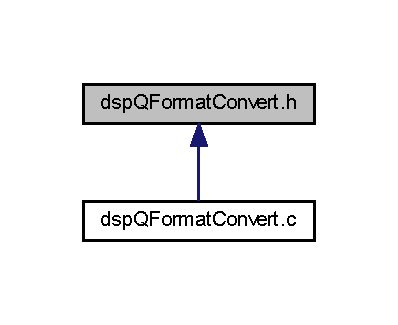
\includegraphics[width=191pt]{d5/dda/dsp_q_format_convert_8h__dep__incl}
\end{center}
\end{figure}
\subsection*{매크로}
\begin{DoxyCompactItemize}
\item 
\#define \hyperlink{dsp_q_format_convert_8h_a4b76a0c2859cfd819a343a780070ee2b}{S\+A\+M\+P\+L\+E\+\_\+\+R\+A\+T\+E}~48000
\begin{DoxyCompactList}\small\item\em Audio Sampling Rate = 48000\+Hz. \end{DoxyCompactList}\item 
\#define \hyperlink{dsp_q_format_convert_8h_a92428112a5d24721208748774a4f23e6}{M\+\_\+\+L\+N2}~0.\+69314718055994530942
\item 
\#define \hyperlink{dsp_q_format_convert_8h_ae71449b1cc6e6250b91f539153a7a0d3}{M\+\_\+\+P\+I}~3.\+14159265358979323846
\begin{DoxyCompactList}\small\item\em Pi Value. \end{DoxyCompactList}\end{DoxyCompactItemize}
\subsection*{함수}
\begin{DoxyCompactItemize}
\item 
int \hyperlink{dsp_q_format_convert_8h_a646289654152ae05600606013b945c86}{Float2\+Q\+Format\+Convert} (\hyperlink{dsp_filter_8h_aeceef54faa278512cd3b46e47d71de18}{\+\_\+\+F\+I\+L\+T\+\_\+\+C\+O\+E\+F} param\+\_\+t\+Filt\+Coef, \hyperlink{dsp_filter_8h_ad441c1c66a421036640642bf5f66b7fa}{\+\_\+\+Q\+\_\+\+F\+O\+R\+M\+A\+T} $\ast$param\+\_\+t\+Filt\+Q\+Form, unsigned int fix\+Num, unsigned int frac\+Num)
\begin{DoxyCompactList}\small\item\em Floating Point Filter Coefficient convert to Fixed Point Q Format Qm.\+n~\newline
. \end{DoxyCompactList}\item 
void \hyperlink{dsp_q_format_convert_8h_a5f03ce0a0de11a675df423d641fe58b2}{Print\+Coef} (int mode, \hyperlink{dsp_filter_8h_aeceef54faa278512cd3b46e47d71de18}{\+\_\+\+F\+I\+L\+T\+\_\+\+C\+O\+E\+F} param\+\_\+t\+Filt\+Coef, \hyperlink{dsp_filter_8h_ad441c1c66a421036640642bf5f66b7fa}{\+\_\+\+Q\+\_\+\+F\+O\+R\+M\+A\+T} param\+\_\+t\+Filt\+Q\+Form, float val\+Freq, float val\+Q, float val\+Gain)
\item 
int \hyperlink{dsp_q_format_convert_8h_a16501f69f57199c5dc647b0fdb9f00bb}{Q\+Format\+Convert} (float param\+\_\+filt\+Coef, int $\ast$param\+\_\+filt\+Q\+Form, unsigned int frac\+Num)
\begin{DoxyCompactList}\small\item\em Q Format Converter Function. \end{DoxyCompactList}\end{DoxyCompactItemize}


\subsection{상세한 설명}
\begin{DoxyDate}{날짜}
2015. 6. 12. 
\end{DoxyDate}
\begin{DoxyAuthor}{작성자}
i04055dt 
\end{DoxyAuthor}


\hyperlink{dsp_q_format_convert_8h_source}{dsp\+Q\+Format\+Convert.\+h} 파일에서 정의되었습니다.



\subsection{매크로 문서화}
\hypertarget{dsp_q_format_convert_8h_a92428112a5d24721208748774a4f23e6}{\index{dsp\+Q\+Format\+Convert.\+h@{dsp\+Q\+Format\+Convert.\+h}!M\+\_\+\+L\+N2@{M\+\_\+\+L\+N2}}
\index{M\+\_\+\+L\+N2@{M\+\_\+\+L\+N2}!dsp\+Q\+Format\+Convert.\+h@{dsp\+Q\+Format\+Convert.\+h}}
\subsubsection[{M\+\_\+\+L\+N2}]{\setlength{\rightskip}{0pt plus 5cm}\#define M\+\_\+\+L\+N2~0.\+69314718055994530942}}\label{dsp_q_format_convert_8h_a92428112a5d24721208748774a4f23e6}


dsp\+Q\+Format\+Convert.\+h 파일의 14 번째 라인에서 정의되었습니다.

\hypertarget{dsp_q_format_convert_8h_ae71449b1cc6e6250b91f539153a7a0d3}{\index{dsp\+Q\+Format\+Convert.\+h@{dsp\+Q\+Format\+Convert.\+h}!M\+\_\+\+P\+I@{M\+\_\+\+P\+I}}
\index{M\+\_\+\+P\+I@{M\+\_\+\+P\+I}!dsp\+Q\+Format\+Convert.\+h@{dsp\+Q\+Format\+Convert.\+h}}
\subsubsection[{M\+\_\+\+P\+I}]{\setlength{\rightskip}{0pt plus 5cm}\#define M\+\_\+\+P\+I~3.\+14159265358979323846}}\label{dsp_q_format_convert_8h_ae71449b1cc6e6250b91f539153a7a0d3}


Pi Value. 



dsp\+Q\+Format\+Convert.\+h 파일의 18 번째 라인에서 정의되었습니다.

\hypertarget{dsp_q_format_convert_8h_a4b76a0c2859cfd819a343a780070ee2b}{\index{dsp\+Q\+Format\+Convert.\+h@{dsp\+Q\+Format\+Convert.\+h}!S\+A\+M\+P\+L\+E\+\_\+\+R\+A\+T\+E@{S\+A\+M\+P\+L\+E\+\_\+\+R\+A\+T\+E}}
\index{S\+A\+M\+P\+L\+E\+\_\+\+R\+A\+T\+E@{S\+A\+M\+P\+L\+E\+\_\+\+R\+A\+T\+E}!dsp\+Q\+Format\+Convert.\+h@{dsp\+Q\+Format\+Convert.\+h}}
\subsubsection[{S\+A\+M\+P\+L\+E\+\_\+\+R\+A\+T\+E}]{\setlength{\rightskip}{0pt plus 5cm}\#define S\+A\+M\+P\+L\+E\+\_\+\+R\+A\+T\+E~48000}}\label{dsp_q_format_convert_8h_a4b76a0c2859cfd819a343a780070ee2b}


Audio Sampling Rate = 48000\+Hz. 



dsp\+Q\+Format\+Convert.\+h 파일의 11 번째 라인에서 정의되었습니다.



\subsection{함수 문서화}
\hypertarget{dsp_q_format_convert_8h_a646289654152ae05600606013b945c86}{\index{dsp\+Q\+Format\+Convert.\+h@{dsp\+Q\+Format\+Convert.\+h}!Float2\+Q\+Format\+Convert@{Float2\+Q\+Format\+Convert}}
\index{Float2\+Q\+Format\+Convert@{Float2\+Q\+Format\+Convert}!dsp\+Q\+Format\+Convert.\+h@{dsp\+Q\+Format\+Convert.\+h}}
\subsubsection[{Float2\+Q\+Format\+Convert}]{\setlength{\rightskip}{0pt plus 5cm}int Float2\+Q\+Format\+Convert (
\begin{DoxyParamCaption}
\item[{{\bf \+\_\+\+F\+I\+L\+T\+\_\+\+C\+O\+E\+F}}]{param\+\_\+t\+Filt\+Coef, }
\item[{{\bf \+\_\+\+Q\+\_\+\+F\+O\+R\+M\+A\+T} $\ast$}]{param\+\_\+t\+Filt\+Q\+Form, }
\item[{unsigned int}]{fix\+Num, }
\item[{unsigned int}]{frac\+Num}
\end{DoxyParamCaption}
)}}\label{dsp_q_format_convert_8h_a646289654152ae05600606013b945c86}


Floating Point Filter Coefficient convert to Fixed Point Q Format Qm.\+n~\newline
. 


\begin{DoxyItemize}
\item Input/\+Output is the Structure of Filter Coefficients \& Q Format Coefficients
\end{DoxyItemize}


\begin{DoxyParams}{매개변수}
{\em param\+\_\+t\+Filt\+Coef} & Src\+: Floating Point Filter Coefficient \\
\hline
{\em param\+\_\+t\+Filt\+Q\+Form} & Des\+: Q Format Integer Filter Coefficient \\
\hline
{\em fix\+Num} & Q Format Fixed Bit Number \\
\hline
{\em frac\+Num} & Q Format Fraction Bit Number \\
\hline
\end{DoxyParams}
\begin{DoxyReturn}{반환값}
No Error\+: 0, Error\+: -\/1 
\end{DoxyReturn}


dsp\+Q\+Format\+Convert.\+c 파일의 33 번째 라인에서 정의되었습니다.



다음을 참조함 \+:  \+\_\+\+\_\+\+F\+I\+L\+T\+\_\+\+C\+O\+E\+F\+::a1, \+\_\+\+\_\+\+Q\+\_\+\+F\+O\+R\+M\+A\+T\+::a1, \+\_\+\+\_\+\+F\+I\+L\+T\+\_\+\+C\+O\+E\+F\+::a2, \+\_\+\+\_\+\+Q\+\_\+\+F\+O\+R\+M\+A\+T\+::a2, \+\_\+\+\_\+\+F\+I\+L\+T\+\_\+\+C\+O\+E\+F\+::b0, \+\_\+\+\_\+\+Q\+\_\+\+F\+O\+R\+M\+A\+T\+::b0, \+\_\+\+\_\+\+F\+I\+L\+T\+\_\+\+C\+O\+E\+F\+::b1, \+\_\+\+\_\+\+Q\+\_\+\+F\+O\+R\+M\+A\+T\+::b1, \+\_\+\+\_\+\+F\+I\+L\+T\+\_\+\+C\+O\+E\+F\+::b2, \+\_\+\+\_\+\+Q\+\_\+\+F\+O\+R\+M\+A\+T\+::b2.

\hypertarget{dsp_q_format_convert_8h_a5f03ce0a0de11a675df423d641fe58b2}{\index{dsp\+Q\+Format\+Convert.\+h@{dsp\+Q\+Format\+Convert.\+h}!Print\+Coef@{Print\+Coef}}
\index{Print\+Coef@{Print\+Coef}!dsp\+Q\+Format\+Convert.\+h@{dsp\+Q\+Format\+Convert.\+h}}
\subsubsection[{Print\+Coef}]{\setlength{\rightskip}{0pt plus 5cm}void Print\+Coef (
\begin{DoxyParamCaption}
\item[{int}]{mode, }
\item[{{\bf \+\_\+\+F\+I\+L\+T\+\_\+\+C\+O\+E\+F}}]{param\+\_\+t\+Filt\+Coef, }
\item[{{\bf \+\_\+\+Q\+\_\+\+F\+O\+R\+M\+A\+T}}]{param\+\_\+t\+Filt\+Q\+Form, }
\item[{float}]{val\+Freq, }
\item[{float}]{val\+Q, }
\item[{float}]{val\+Gain}
\end{DoxyParamCaption}
)}}\label{dsp_q_format_convert_8h_a5f03ce0a0de11a675df423d641fe58b2}
Print Filter Coefficient Floating Value And Q1.\+31 Format 
\begin{DoxyParams}{매개변수}
{\em mode} & E\+Q Filter Mode~\newline

\begin{DoxyItemize}
\item 0\+: Low Pass Shelving Filter~\newline

\item 1\+: High Pass Shelving Filter~\newline

\item 2\+: Peak Filter~\newline

\item 3\+: Parametric E\+Q Filter~\newline

\item 4\+: 1st order Low Pass Shelving Filter 
\end{DoxyItemize}\\
\hline
{\em param\+\_\+t\+Filt\+Coef} & \\
\hline
{\em param\+\_\+t\+Filt\+Q\+Form} & \\
\hline
{\em val\+Freq} & \\
\hline
{\em val\+Q} & \\
\hline
{\em val\+Gain} & \\
\hline
\end{DoxyParams}


dsp\+Q\+Format\+Convert.\+c 파일의 101 번째 라인에서 정의되었습니다.



다음을 참조함 \+:  \+\_\+\+\_\+\+F\+I\+L\+T\+\_\+\+C\+O\+E\+F\+::a1, \+\_\+\+\_\+\+Q\+\_\+\+F\+O\+R\+M\+A\+T\+::a1, \+\_\+\+\_\+\+F\+I\+L\+T\+\_\+\+C\+O\+E\+F\+::a2, \+\_\+\+\_\+\+Q\+\_\+\+F\+O\+R\+M\+A\+T\+::a2, \+\_\+\+\_\+\+F\+I\+L\+T\+\_\+\+C\+O\+E\+F\+::b0, \+\_\+\+\_\+\+Q\+\_\+\+F\+O\+R\+M\+A\+T\+::b0, \+\_\+\+\_\+\+F\+I\+L\+T\+\_\+\+C\+O\+E\+F\+::b1, \+\_\+\+\_\+\+Q\+\_\+\+F\+O\+R\+M\+A\+T\+::b1, \+\_\+\+\_\+\+F\+I\+L\+T\+\_\+\+C\+O\+E\+F\+::b2, \+\_\+\+\_\+\+Q\+\_\+\+F\+O\+R\+M\+A\+T\+::b2, str1st\+Lo\+Shelf\+Filter, str2nd\+Hi\+Shelf\+Filter, str2nd\+Lo\+Shelf\+Filter, str\+Peak\+Filter, str\+Peq\+Filter.

\hypertarget{dsp_q_format_convert_8h_a16501f69f57199c5dc647b0fdb9f00bb}{\index{dsp\+Q\+Format\+Convert.\+h@{dsp\+Q\+Format\+Convert.\+h}!Q\+Format\+Convert@{Q\+Format\+Convert}}
\index{Q\+Format\+Convert@{Q\+Format\+Convert}!dsp\+Q\+Format\+Convert.\+h@{dsp\+Q\+Format\+Convert.\+h}}
\subsubsection[{Q\+Format\+Convert}]{\setlength{\rightskip}{0pt plus 5cm}int Q\+Format\+Convert (
\begin{DoxyParamCaption}
\item[{float}]{param\+\_\+filt\+Coef, }
\item[{int $\ast$}]{param\+\_\+filt\+Q\+Form, }
\item[{unsigned int}]{frac\+Num}
\end{DoxyParamCaption}
)}}\label{dsp_q_format_convert_8h_a16501f69f57199c5dc647b0fdb9f00bb}


Q Format Converter Function. 


\begin{DoxyParams}{매개변수}
{\em param\+\_\+filt\+Coef} & Src\+: Floating Point Filter Coefficient \\
\hline
{\em param\+\_\+filt\+Q\+Form} & Des\+: Q Format Integer Filter Coefficient \\
\hline
{\em frac\+Num} & Q Format Fraction Bit Number (n number of Qm.\+n format) \\
\hline
\end{DoxyParams}
\begin{DoxyReturn}{반환값}
Error -\/1, Normal\+: 0 
\end{DoxyReturn}


dsp\+Q\+Format\+Convert.\+c 파일의 181 번째 라인에서 정의되었습니다.


\hypertarget{xmos___hello_world_8xc}{\section{xmos\+\_\+\+Hello\+World.\+xc 파일 참조}
\label{xmos___hello_world_8xc}\index{xmos\+\_\+\+Hello\+World.\+xc@{xmos\+\_\+\+Hello\+World.\+xc}}
}

%--- End generated contents ---

% Index
\newpage
\phantomsection
\addcontentsline{toc}{chapter}{색인}
\printindex

\end{document}
